\section{Implementation Details}
\label{implementationdetails}
The new~\texttt{vtkGPUVolumeRayCastMapper} uses a ray casting
technique~\citep{engel_real-time_2006} for volume rendering which is
state-of-the-art on modern graphics platforms. At a high level, it is similar to
the previous version of this class, with a different OpenGL implementation
reflecting recent advances in graphics systems. One of the main reasons we chose
to use ray casting is due to the flexibility of this technique, which supports the
many features of the previous software ray cast mapper but with the acceleration
of the GPU. Ray casting is an image-order rendering technique, with one or more
rays cast through the volume per image pixel. VTK is inherently an object-order
rendering system, where the GPU renders all graphical primitives (points, lines,
triangles, etc.) represented by instances of vtkProp in a scene using one or
more rendering passes (with multiple passes needed to support advanced features
such as depth peeling for transparency).

The image-order rendering process for vtkVolume is initiated when the
front-facing polygons of the volume’s bounding box are rendered with a custom
fragment program. This fragment program is used to cast a ray through the volume
at each pixel, with the fragment location indicating the starting location for
that ray. The volume and all the various rendering parameters are transferred to
the GPU through the use of textures (3D for the volume, 1D for the various
transfer functions) and uniform variables. Steps are taken along the ray until
the ray exits the volume, and the resulting computed color and opacity are
blended into the current pixel value. Note that volumes are rendered after rendering opaque geometry, to allow the ray casting process to terminate at
the depth value stored in the depth buffer for that pixel (and hence correctly
intermix with opaque geometry).

In addition to providing supported features of the old mapper, the new mapper
adds new capabilities such as GPU-based clipping,  gradient opacity, and volume
picking amongst many others. In the next few sections, we will cover each of
these features in detail.

\subsection{Single Pass}
% \begin{figure}[ht]
%   \centering
%   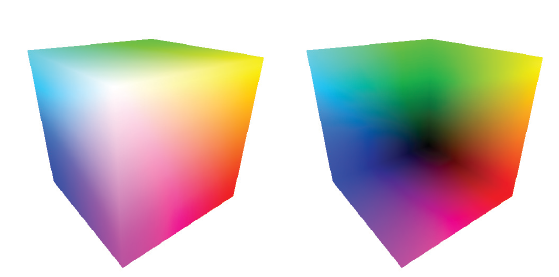
\includegraphics[width=\columnwidth]{frontandback.png}
%   \caption{Front and back faces are rendered for start and end position of the
%   ray.}
%   \label{fig:frontandback}
% \end{figure}%


% \begin{figure}[ht]
%   \centering
%   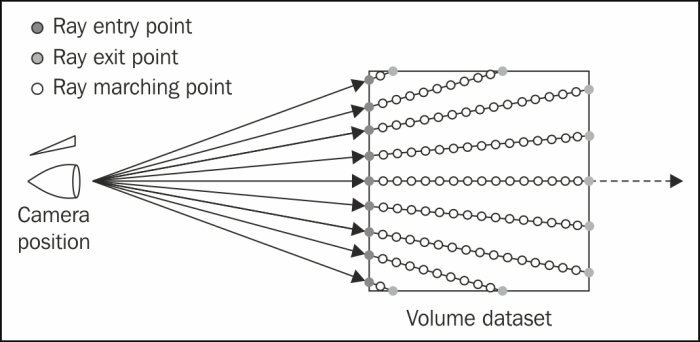
\includegraphics[width=\columnwidth]{raycasting}
%   \caption{Implementing volume rendering using single-pass GPU ray casting.}
%   \label{fig:raycasting}
% \end{figure}%

In a ray-casting algorithm, the entry and the exit point into the volume is
needed to determine when to stop ray stepping process. To determine the entry and
the exit point, one approach is to render the geometry of the volume bounding
box of the volume twice. In the first pass, the front face of the geometry is
rendered and in the second pass the back face is rendered.
% as shown in ~\Autoref{fig:frontandback}.
Using the interpolated vertex position and
texture lookup, the start and end positions can be computed. Instead of this, in
\texttt{vtkGPUVolumeRayCastMapper}, entry and exit points are computed based on
the fact that the texture extents of the volume are within vec3(1.0), vec3(-1.0)
range.% (as shown in ~\Autoref{fig:raycasting}).
The code below shows the
fragment shader pseudo code that determines whether or not to stop ray stepping
through the volume.

\begin{center}
  \begin{lstlisting}[language=Python, caption={Ray stop determination},
                     captionpos=b, frame=single, breaklines=true]
bool stop = any(greaterThan(g_dataPos,
                            ip_texMax)) ||
            any(lessThan(g_dataPos,
                         ip_texMin));
  \end{lstlisting}
\end{center}

The advantage of such approach is that it requires one less pass, and is faster
than other approaches since there is no texture generation or lookup required
to determine the termination of the ray.


\subsection{Dynamic Shader Generation}
All operations are performed on the GPU in the
new~\texttt{vtkOpenGLGPUVolumeRayCastMapper}. The advantage of this approach is
more streamlined code that is easier to maintain and debug. This approach also
provides an opportunity to rework how to support different features without
having too many branches in the shader code or having to send all the options to
the shader because that would have been detrimental for performance. In this
improved mapper, the shader is dynamically composed by the mapper. For this to
work, we have introduced tags in a vertex or fragment shader which are then
replaced by the~\texttt{vtkVolumeShaderComposer} depending on the options
enabled or chosen by the application code. These tags correspond to each setup
in a ray casting shader: 1) Declaration of variables 2) Initialization of ray
position and direction 3) Iterative Ray traversal inside the volume and check
for ray termination conditions 4) Final color and opacity computation after ray
termination.% For instance, the skeleton fragment shader defines tags as shown
%in~\Autoref{lst:skeletonshader}.

%\begin{lstlisting}[language=C++, caption={Fragment shader tags},
                   %captionpos=b, frame=single, breaklines=true,
                   %label=lst:skeletonshader]

%int main()
%{
  %// The tag below will be replaced by a
  %// a concatenated string at run-time that
  %// declares the appropriate core
  %// shader variables which will be used regardless
  %// of the operation (MIP, MinIP) performed.
  %// The replacement is shown in ~\Autoref{lst:basedeclshader}.
  %//VTK::Base::Dec

  %// The tag below will be replaced to declare
  %// variables that are responsible for termination
  %// of the ray-casting. Essentially this enables
  %// users to partially replace the shader and customize
  %// it as necessary.
  %//VTK::Termination::Dec

  %// Advance ray and accumulate color and opacity
  %while(not exit)
  %{
    %// This tag will be replaced by a concatenated
    %// string that performs color and opacity aggregation
    %// along the ray.
    %//VTK::Base::Impl

    %// Other tags implementing Cropping, Clipping etc.

    %// Advance ray here

    %// This tag will be replaced by a concatenated
    %// string that will check if the ray is still
    %// inside the volume and other checks.
    %//VTK::Terminate::Impl
  %}

  %// This tag will be replaced by a concatenated
  %// string that performs final color, depth, and opacity
  %// computation.
  %//VTK::Shading::Exit
%}

%\end{lstlisting}

To define a structure, we have chosen a strategy that separates the tags in
the following four categories:

\begin{enumerate}
\label{enu:shadertags}
  \item \textbf{Declaration (::Dec)} The tags belonging to this group are meant
    to declare variables or function outside the main execution of the shader
    code.  The variables defined are uniform, varying, and user-defined global
    variables.  The functions defined are typically perform operations that are
    repetitive in nature such as computing color of a fragment.

  \item \textbf{Initialization (::Init)} The tags belonging to this group are
    meant to initialize variables inside the main execution function of the
    shader but before the ray-casting loop in the fragment shader. An example of
    such code includes computation of ray initial position and direction
    of traversal.

  \item \textbf{Implementation (::Impl)} The tags belonging to this group are
    the variables or functions or the combination of both that perform the
    actual operation of clipping, cropping, shading, etc. on one, two, or four
    component volume data.  The implementation code uses local and global
    variables and is optimized for performance reasons as it is executed as long
    as the ray is traversing inside the volume and didn't run into a termination
    condition which is checked every time.

  \item \textbf{Exit (::Exit)} The tags belonging to this group perform final
    computation such as the final color of the fragment. These tags are placed
    outside the ray-casting loop and typically contain numeric assignments.
\end{enumerate}

\subsection{Lighting / Shading}
\label{lighting}
The old mapper supported only one light (due to limitations in OpenGL at the
time the class was written). Similarly
the~\texttt{vtkFixedPointVolumeRayCastMapper} supports multiple lights, but only
with an approximate lighting model, since gradients are precomputed and
quantized, and shading is performed for each potential gradient direction
regardless of fragment location. However the new mapper accurately implements
the VTK lighting model to produce high quality images for publication. To
support this, depending on the light type (point, directional, and positional),
the lighting parameters are sent to the shader which then performs the per pixel
lighting calculations. The number of lights is limited to six, mostly for
performance reasons as the interactive frame rate goes down significantly with
each light added to the scene. The Phong shading lighting model is used for
volume rendering lighting. Phong lighting requires normals which must be
computed for each fragment. The normal calculation is done by first computing
the gradient and then scaling the gradient by the spacing between the cells. The
gradient is computed by reading the scalar values form the neighboring cells
using the offset vector that stores the step size based on the bounds of the
volume.

\subsection{Volume Picking}
\label{picking}
Picking, in the context of volume rendering, is the action of resolving the set
of voxels a user has clicked on with the pointer. This provides the user with the
means to interact with objects in a 3D scene. VTK legacy volume mappers
support picking through an instance external to the mapper itself
called~\texttt{vtkVolumePicker}.  This class casts a ray into the volume and
returns the point where the ray intersects an isosurface of a user specified
opacity.  This technique has certain limitations given that the picking class
does not have enough information to correctly account for clipping, transfer
functions, and other parameters defining how the mapper renders, thus
reducing its reliability on the objects being picked.

Now VTK supports hardware-accelerated picking of geometric data through the
class~\texttt{vtkHardwareSelector}, which uses a multiple-render-pass approach
in order to resolve the various objects in a scene (actors or props in VTK
parlance) and their corresponding primitives.  Each pass renders separately a
different selection abstraction (processes, actors, composite blocks and
primitives), painting with a different color each of the various components in
the scene.  The images rendered by each pass are downloaded from the GPU and
subsequently analyzed in the class thereby resolving the correspondence of each
pixel to its particular actor, primitive, etc.

The inherent flexibility of the revamped shader implementation of this mapper
permits a seamless integration with~\texttt{vtkHardwareSelector}'s interface by
rendering the appropriate colors for each of its passes, hence granting
consistency in the object selection regardless of whether it is geometric or
volumetric data.  Providing selection support directly within the fragment
shader ensures high selection accuracy even in situations where a volume
intermixes with geometry in seemingly cumbersome ways, or other advanced features
(e.g. clipping) are enabled (what you see is what you pick).  Given the readily
available picking styles supported by~\texttt{vtkHardwareSelector}
(e.g.~\texttt{vtkAreaPicker}), it is possible to make a selection of a specific
set of visible voxels.

\subsection{Volume Texture Streaming}
\label{streaming}
A common limitation of volume rendering is that the 3D volume data does not
always fit into the graphics memory of a system. This limitation has become
increasingly important to address as the new mapper provides support for mobile
architectures.  A relatively simple method when dealing with a large volume is
the volume streaming approach also commonly known as
bricking~\citep{engel_real-time_2006} in which the volume is split into several
blocks so that a single sub-block (brick) fits completely into GPU memory.  Each
sub-block is stored in main memory and streamed into GPU memory for a rendering
pass one at a time (in a back-to-front manner for correct composition). The
sub-blocks are rendered using the standard shader programs and alpha-blended
with each other by OpenGL. Streaming the volume as separate texture bricks
certainly imposes a performance trade-off but acts as a graphics memory
expansion scheme for devices that are not able to render a large volume
otherwise.

\subsection{Dual Depth-Peeling}
\label{peeling}
VTK has long supported the use of depth-peeling for order-independent rendering
of translucent geometry. Since translucent fragments must be blended in a
specific order to obtain the correct pixel color, techniques like depth-peeling
are necessary for correctly shading a complex scene.

In a multipass depth-peeling rendering, `slices' of fragments are pulled from
the scene in depth order; the nearest fragments per pixel are collected in
the first pass, and then the fragments just behind those are written in the next
pass. After each pass, the current set of fragments is blended into an
accumulation buffer, ultimately producing a correctly colored scene in which all
fragments are blended front-to-back.

The standard depth-peeling algorithm, which collects a single layer of fragments
per geometry pass in front-to-back order, was recently updated to use a ``dual
depth-peeling'' technique~\citep{bavoil_order_2008}, in which two layers of
fragments are peeled in a single geometry pass: one layer from the front and a
second from the back. These are blended into two separate accumulation buffers,
and eventually the front and back peels meet towards the middle of the
geometry. This allows depth-peeling to be carried out in roughly half as many
geometry passes.  For this purpose, accumulation buffers have been implemented
as RGBA8 texture attachments of a framebuffer to which the rendering results
are output on each intermediate peeling/blending pass.

An interesting detail of the new depth-peeling implementation is that there are
four depth values available per-pixel during a typical peeling pass. Two depth
values each are associated with the front and back peels; these are the depth of
the currently peeled fragment, and the depth of the next fragment that will be
peeled. These depth values can be reinterpreted as two sets of ``inner'' and
``outer'' boundaries for a view-ray traversing a volume.

By adapting the volume mapper's fragment shader to use these depth values for
computing two ``slices'' of a volume, we are able to integrate volume rendering
into our depth-peeling pass. This enables volumetric data to be mixed with
translucent geometry while efficiently yielding a correctly colored result
~\Autoref{fig:volume_peeling_tooth}.

\begin{figure}[ht]
\centering
  \begin{subfigure}[b]{.5\columnwidth}
    \centering
    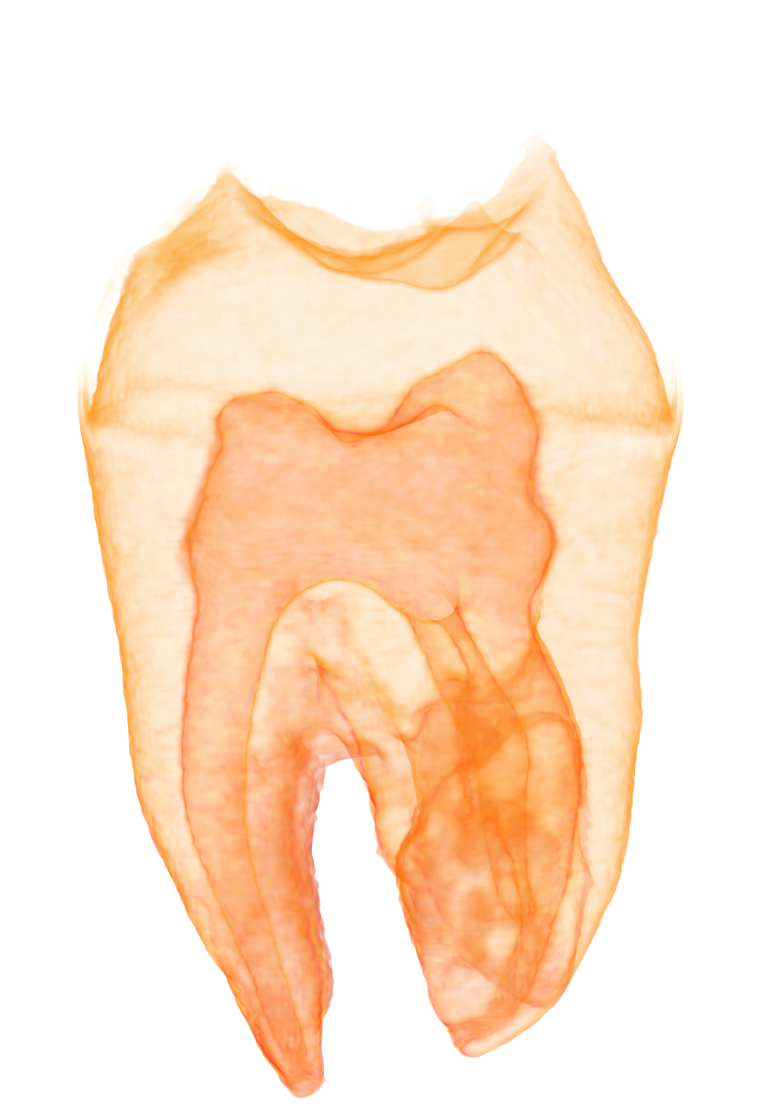
\includegraphics[width=\columnwidth]{tooth_front_}
    \caption{Volume only}
    \label{fig:tooth_front}
  \end{subfigure}%
  \begin{subfigure}[b]{.5\columnwidth}
    \centering
    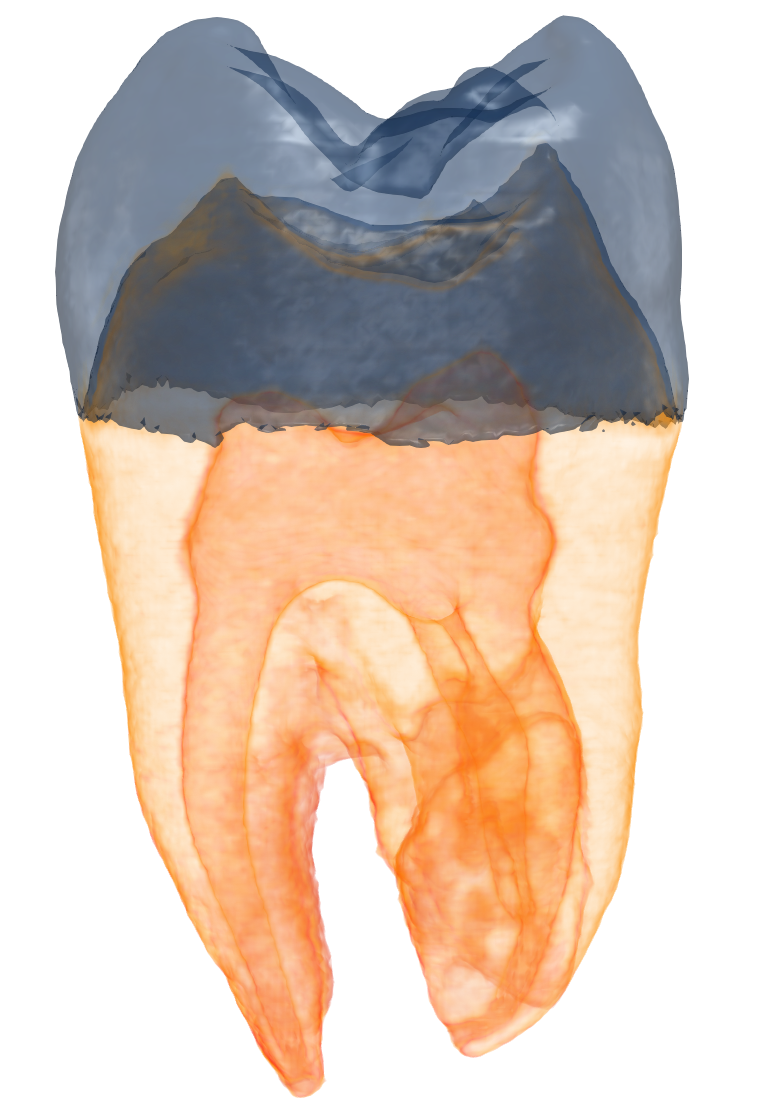
\includegraphics[width=\columnwidth]{tooth_front_enamel}
    \caption{Intermixed}
    \label{fig:tooth_front_enamel}
  \end{subfigure}
  \begin{subfigure}[b]{.5\columnwidth}
    \centering
    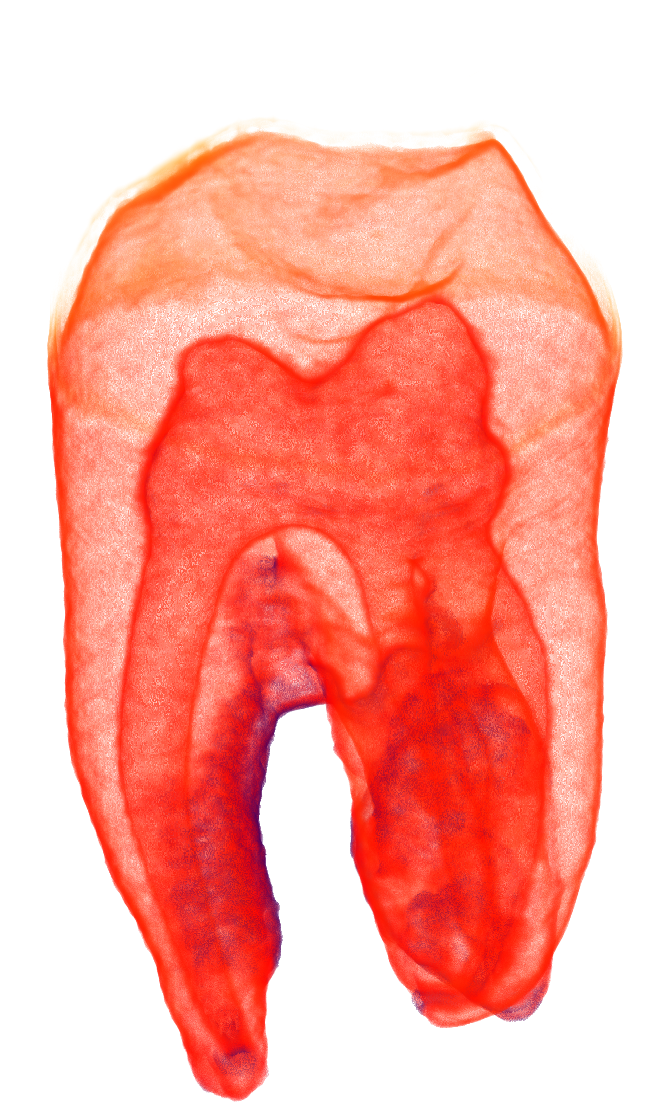
\includegraphics[width=\columnwidth]{tooth_bottom_}
    \caption{Volume only (rotated)}
    \label{fig:tooth_bottom}
  \end{subfigure}%
  \begin{subfigure}[b]{.5\columnwidth}
    \centering
    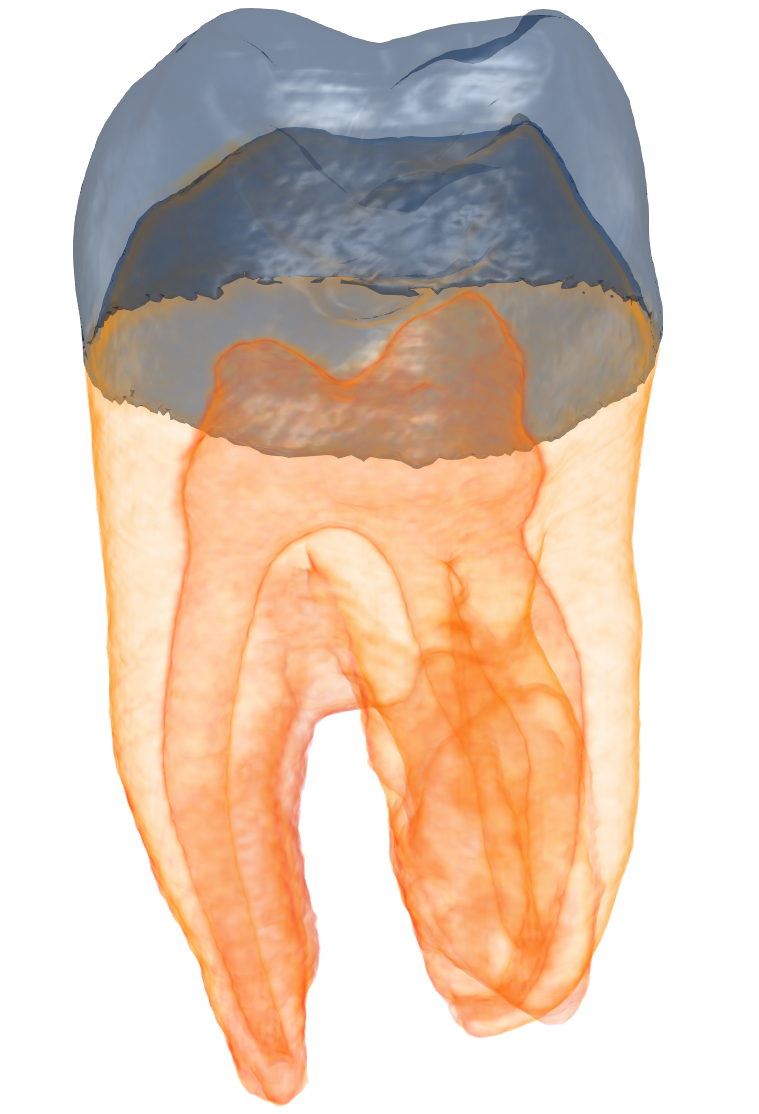
\includegraphics[width=\columnwidth]{tooth_bottom_enamel}
    \caption{Intermixed (rotated)}
    \label{fig:tooth_bottom_enamel}
  \end{subfigure}
  \caption{Industrial CT scan of a human tooth~\citep{pfister_transfer_2001}.
    The dentin and pulp of the tooth are rendered as a volume (a) while an
    iso-contour of the enamel is rendered as translucent polygonal geometry (b).
    (c) and (d) show a different viewpoint (object rotated on the horizontal axis)
    from which it is easier to observe the correct ordering of the rendered
    entities.}
  \label{fig:volume_peeling_tooth}
\end{figure}

\subsection{Render to Texture}
\label{rendertotexture}
Typically, the mapper uses a single pass
rendering approach in which the 3D volume data is rendered on screen i.e. the
default framebuffer that comprises of a color and a depth buffer. In games and
other graphics applications, a multi-pass rendering approach called ``Render to
Texture'' is used to support advanced visual rendering techniques such as
deferred shading, texture baking, post processing, etc. This technique uses the
rendered output from one pass to modify/enhance the output of other rendering
passes.

\begin{figure}[ht]
\centering
  \begin{subfigure}[b]{.5\columnwidth}
    \centering
    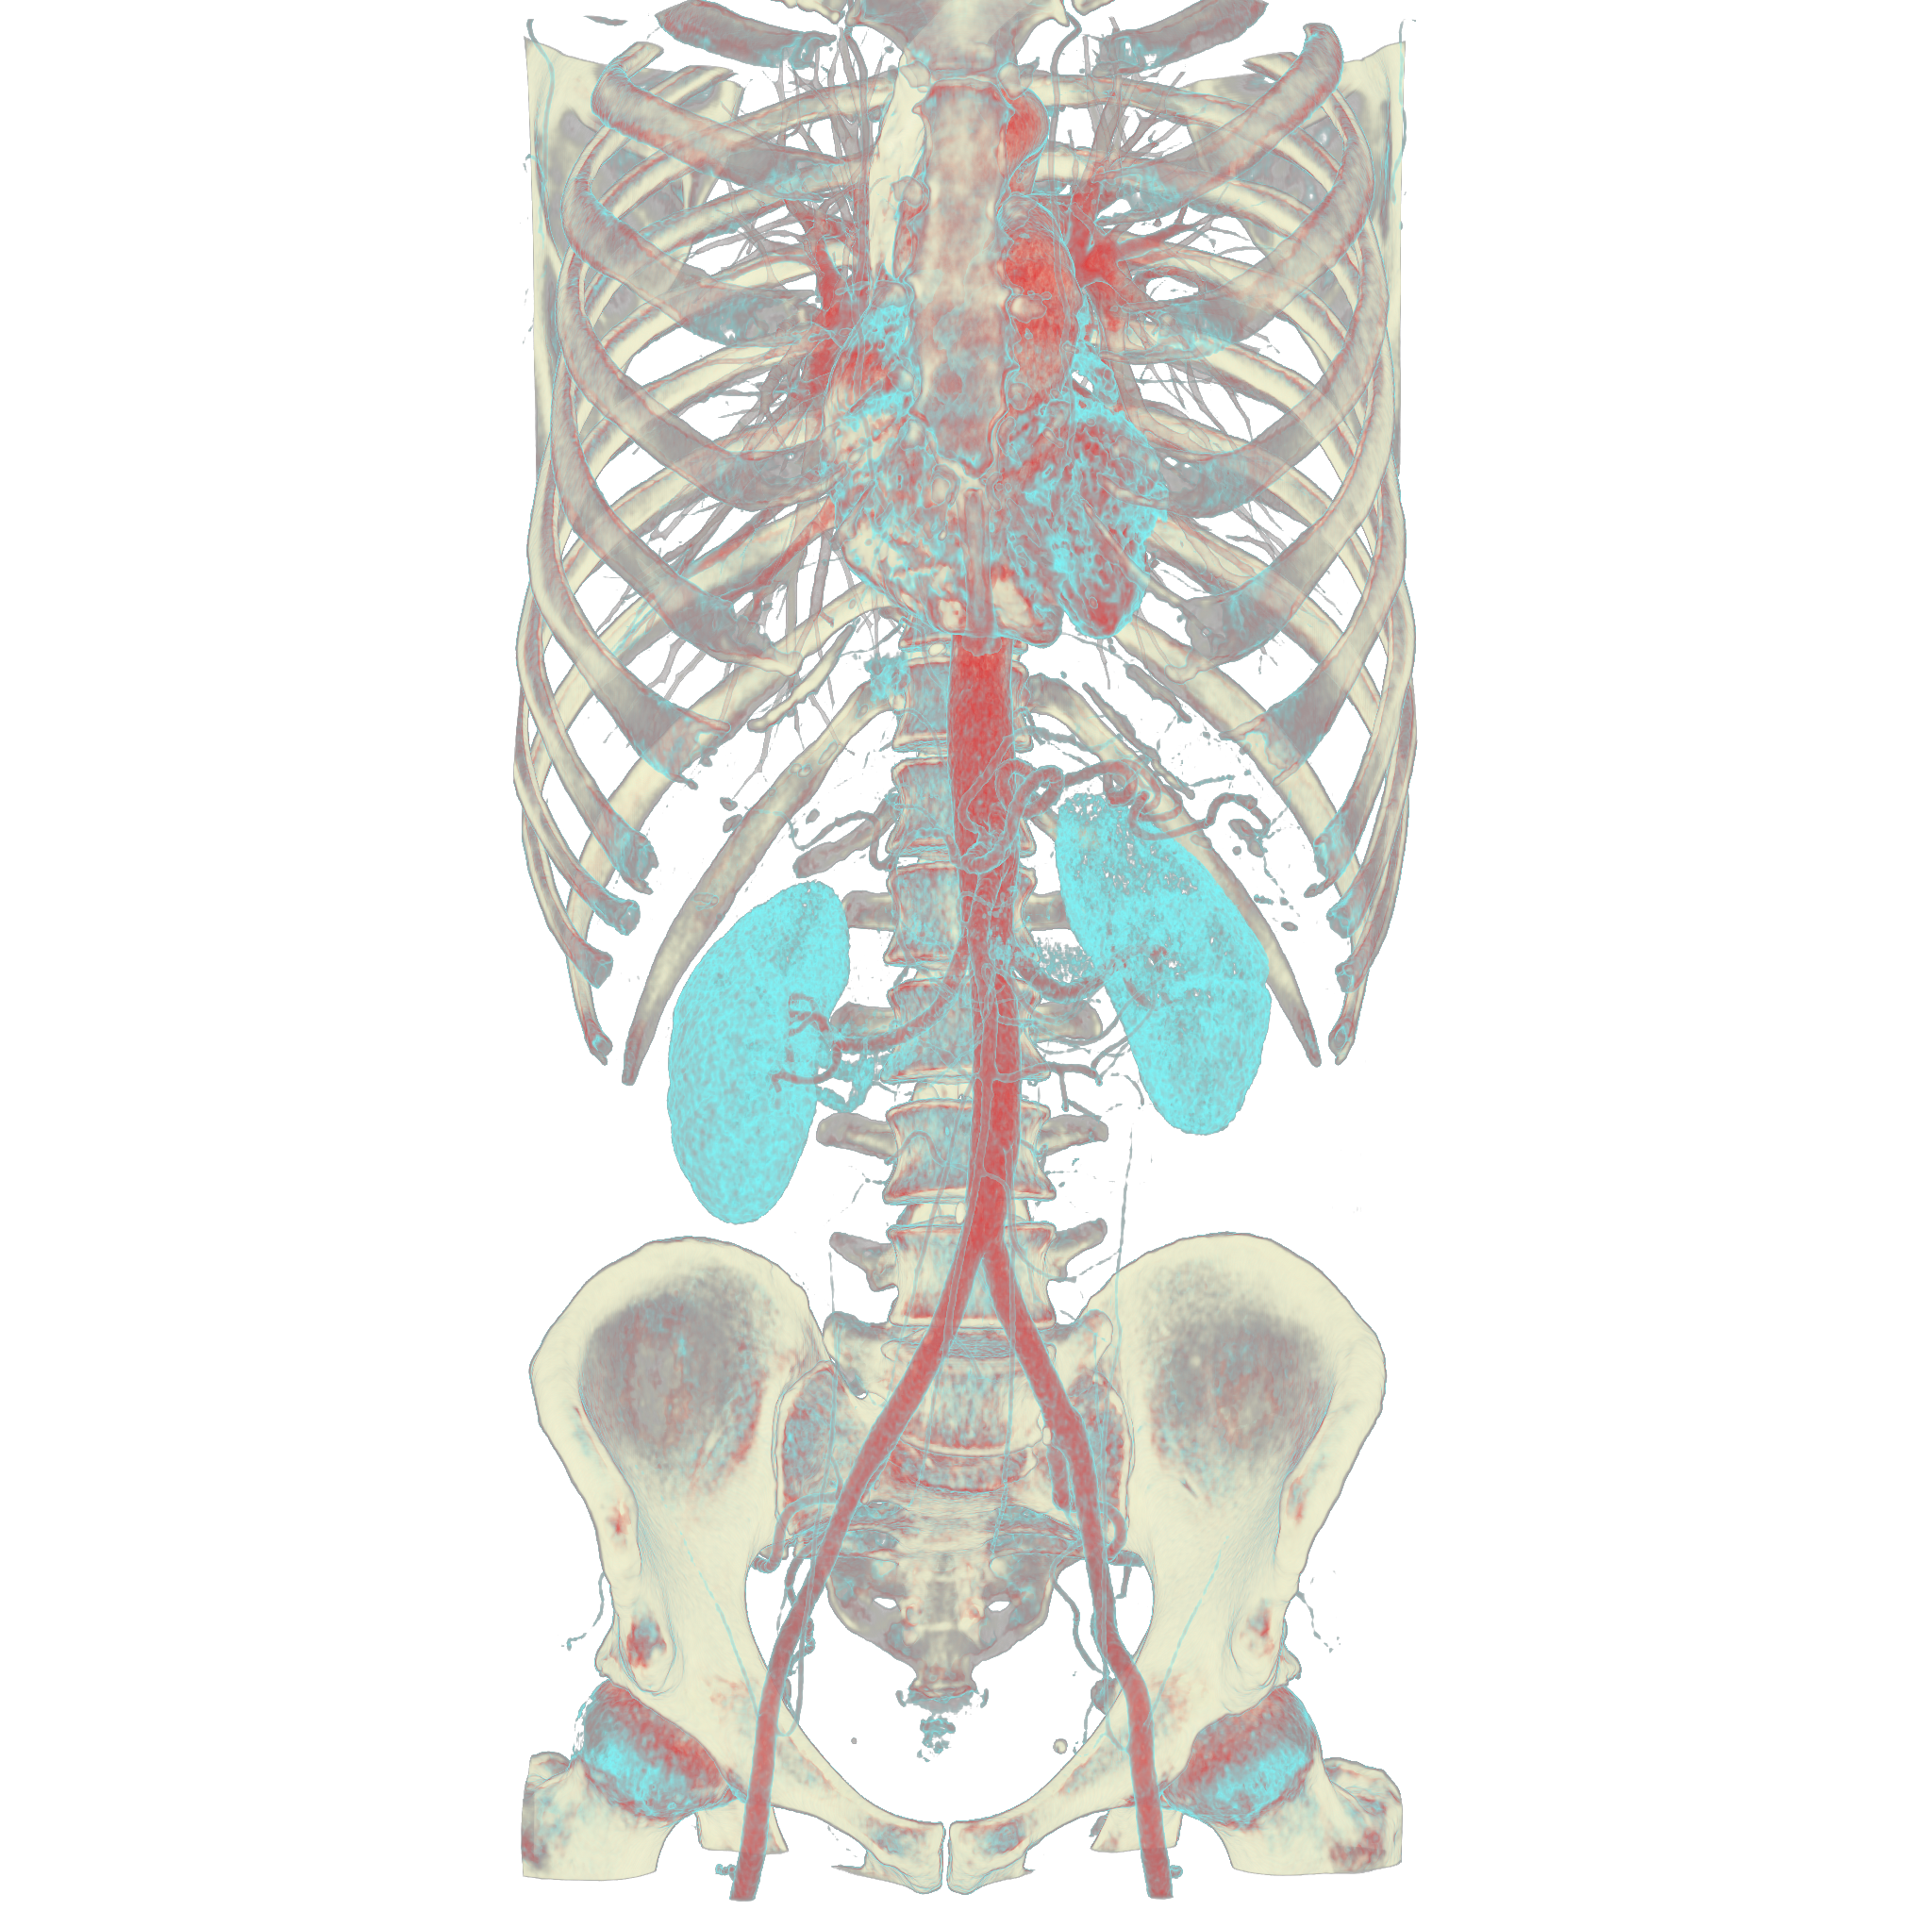
\includegraphics[width=\columnwidth]{colorimage}
    \caption{Color image}
    \label{fig:rendertotexturecolor}
  \end{subfigure}%
  \begin{subfigure}[b]{.5\columnwidth}
    \centering
    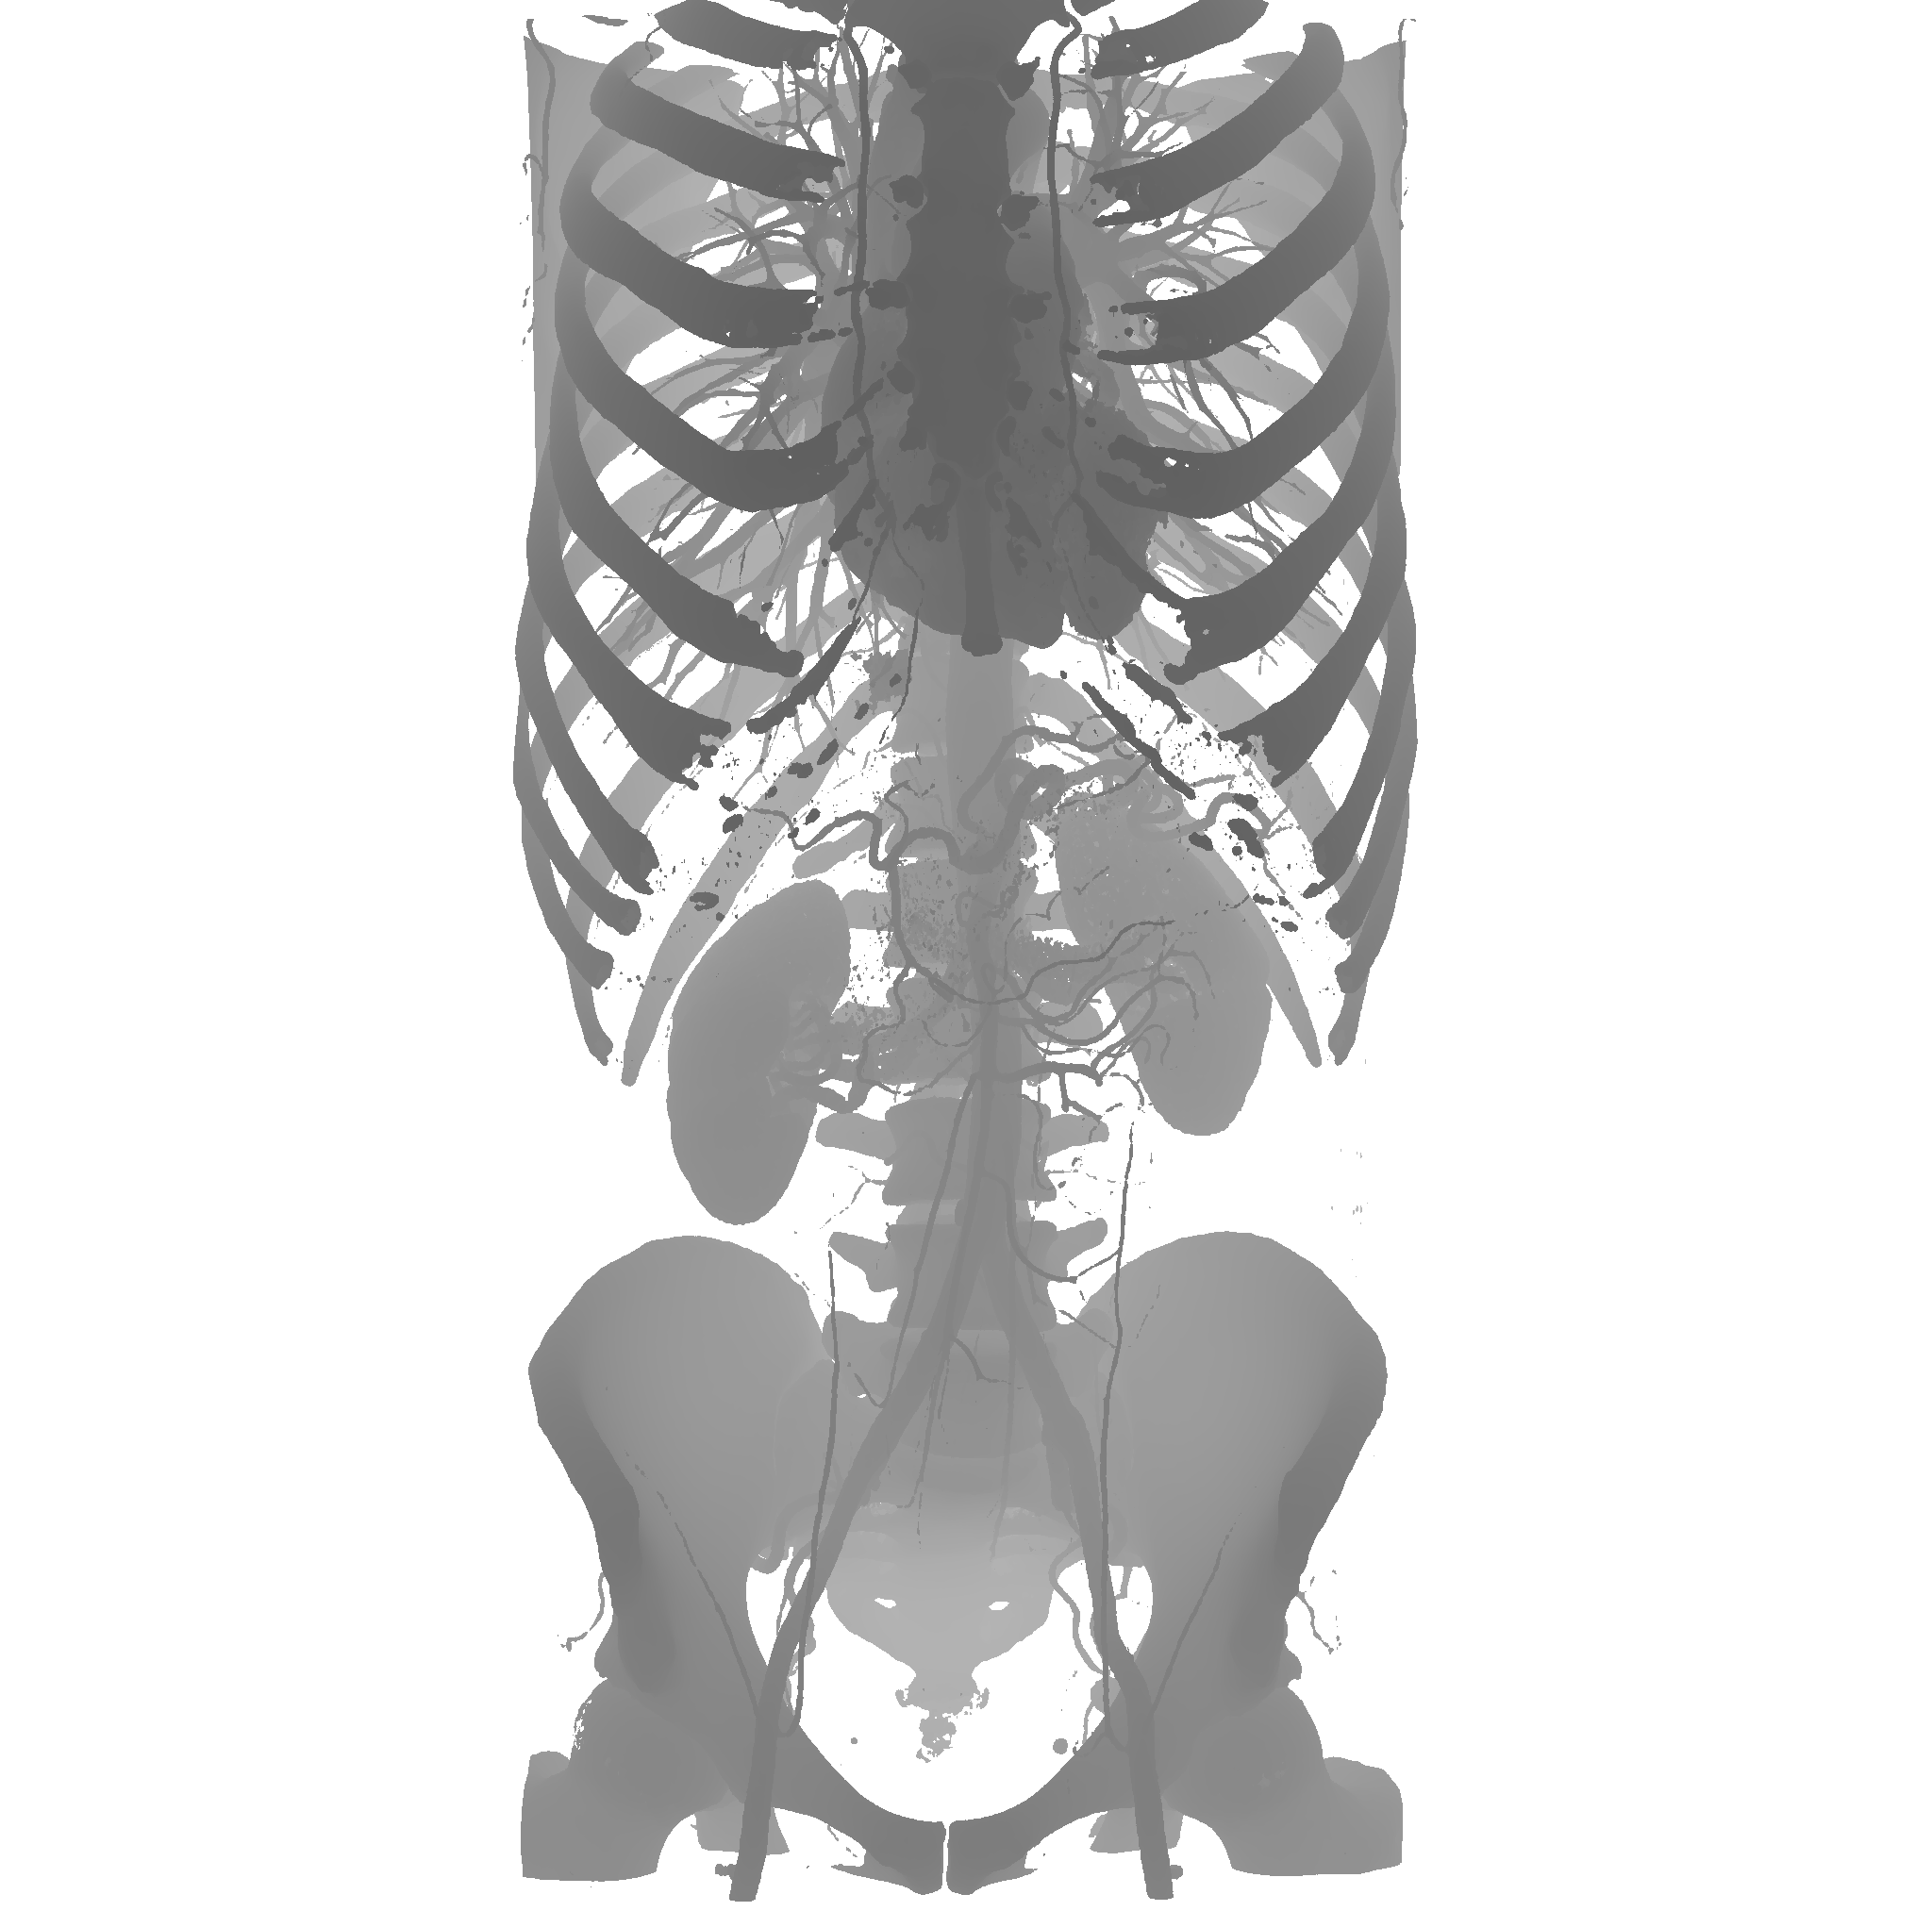
\includegraphics[width=\columnwidth]{depthimage}
    \caption{Depth image}
    \label{fig:rendertotexturedepth}
  \end{subfigure}
  \caption{When~\texttt{RenderToImage} is enabled, the color and depth data of
    the final rendering is written to a texture object which can be used for
    further processing}
  \label{fig:rendertotexture}
\end{figure}

When the \texttt{RenderToImage} flag is enabled, the volume mapper switches
rendering to an OpenGL FrameBufferObject (FBO) and allows the user to obtain the
rendered pixel data via simple image retrieval calls. The mapper provides
methods to grab color and depth information either as individual textures or as
VTK's image data structure -~\texttt{vtkImageData}. The color data is simply the
pixel representation of the rendered volume whereas depth data consists of a
grayscale image depicting how deep each voxel is in the scene (as depicted
in~\Autoref{fig:rendertotexture}). When an application enables render-to-texture
mode, a framebuffer object is created, the vertex and fragment shader are
generated, color and depth buffers are cleared, and the color is set to white
with a value of zero alpha. The value of zero alpha is used so that applications
can safely ignore the transparent pixels, and the color buffer is set to white
color because white represents the maximum depth: the depth of the far
plane. In the render-to-texture pass, the fragment shader writes to color and
depth target. To write the depth information it uses the depth of the first
non-transparent voxel.

\subsection{Stochastic Jittering}
\label{jittering}
Because ray-casting effectively samples a discrete signal (voxel values along
the ray trajectory), the distance between sampling points heavily influences how
accurately the volume data is represented.  Due to well established limitations
described by the sampling theorem, low sampling rates may result in aliasing
effects often referred to as wood-grain artifacts as shown
in~\Autoref{fig:jittering_without} in the context of volume
rendering~\citep{engel_real-time_2006}. Reducing the distance between samples
neutralizes these artifacts but takes an important toll on performance.

The mapper supports stochastic jittering, which is an alternative technique to
counteract wood-grain artifacts by adding a random offset to the rays in the
viewing direction thereby breaking the coherence between neighboring fragments
which causes the aliased patterns become less apparent as shown
in~\Autoref{fig:jittering_with}.  Jittering is implemented by creating a random
noise texture (using~\texttt{vtkPerlinNoise}) and applying the offset to the
ray's starting point, resulting in a much lower performance penalty than reducing
the sampling distance.

\begin{figure}[htb]
\centering
  \begin{subfigure}[b]{.5\columnwidth}
    \centering
    \includegraphics[width=\textwidth]{cactus_holland_woodgrain}
    \caption{Wood-grain artifacts.}
    \label{fig:jittering_without}
  \end{subfigure}%
  \begin{subfigure}[b]{.5\columnwidth}
    \centering
    \includegraphics[width=\textwidth]{cactus_holland_jittering}
    \caption{Jittering enabled.}
    \label{fig:jittering_with}
  \end{subfigure}
  \caption{Cactus sample scanned at Beamline 8.3.2, Advanced Light Source,
    Lawrence Berkeley National Laboratory. A coarse ray-sampling distance causes
    wood-grain artifacts~(a) to appear. Same data and sampling distance with
    stochastic jittering enabled~(b) to mitigate the artifacts.}
  \label{fig:jittering}
\end{figure}

\subsection{Clipping}
\label{clipping}
A set of infinite planes can be defined to clip the volume to reveal inner
detail, as shown in Figure 4.  The visibility of each sample along the ray
is determined by computing the sample's distance to each plane and testing
for it being in front or behind.

The current implementation iterates through each of the planes before entering
the ray marching loop in order to early-discard rays which meet any of the
following criteria:

\begin{enumerate}
\item Entering the volume on the clipped side and exiting before ever
  intersecting the plane (the ray only traverses clipped space).
\item Intersecting overlapping geometry before the plane (z-buffer compositing).
\end{enumerate}

\subsection{Cropping}
\label{cropping}
Cropping refers to the 27 regions defined by pairs of
planes along each volume coordinate axis and can be independently turned
on (visible) or off (invisible) to produce a variety of different cropping
effects%, as shown in ~\Autoref{fig:cropping}.
Cropping is implemented by determining the cropping region of each sample
location along the ray and including only those samples that fall within
a visible region.

% \begin{figure}[htb]
%   \centering
%   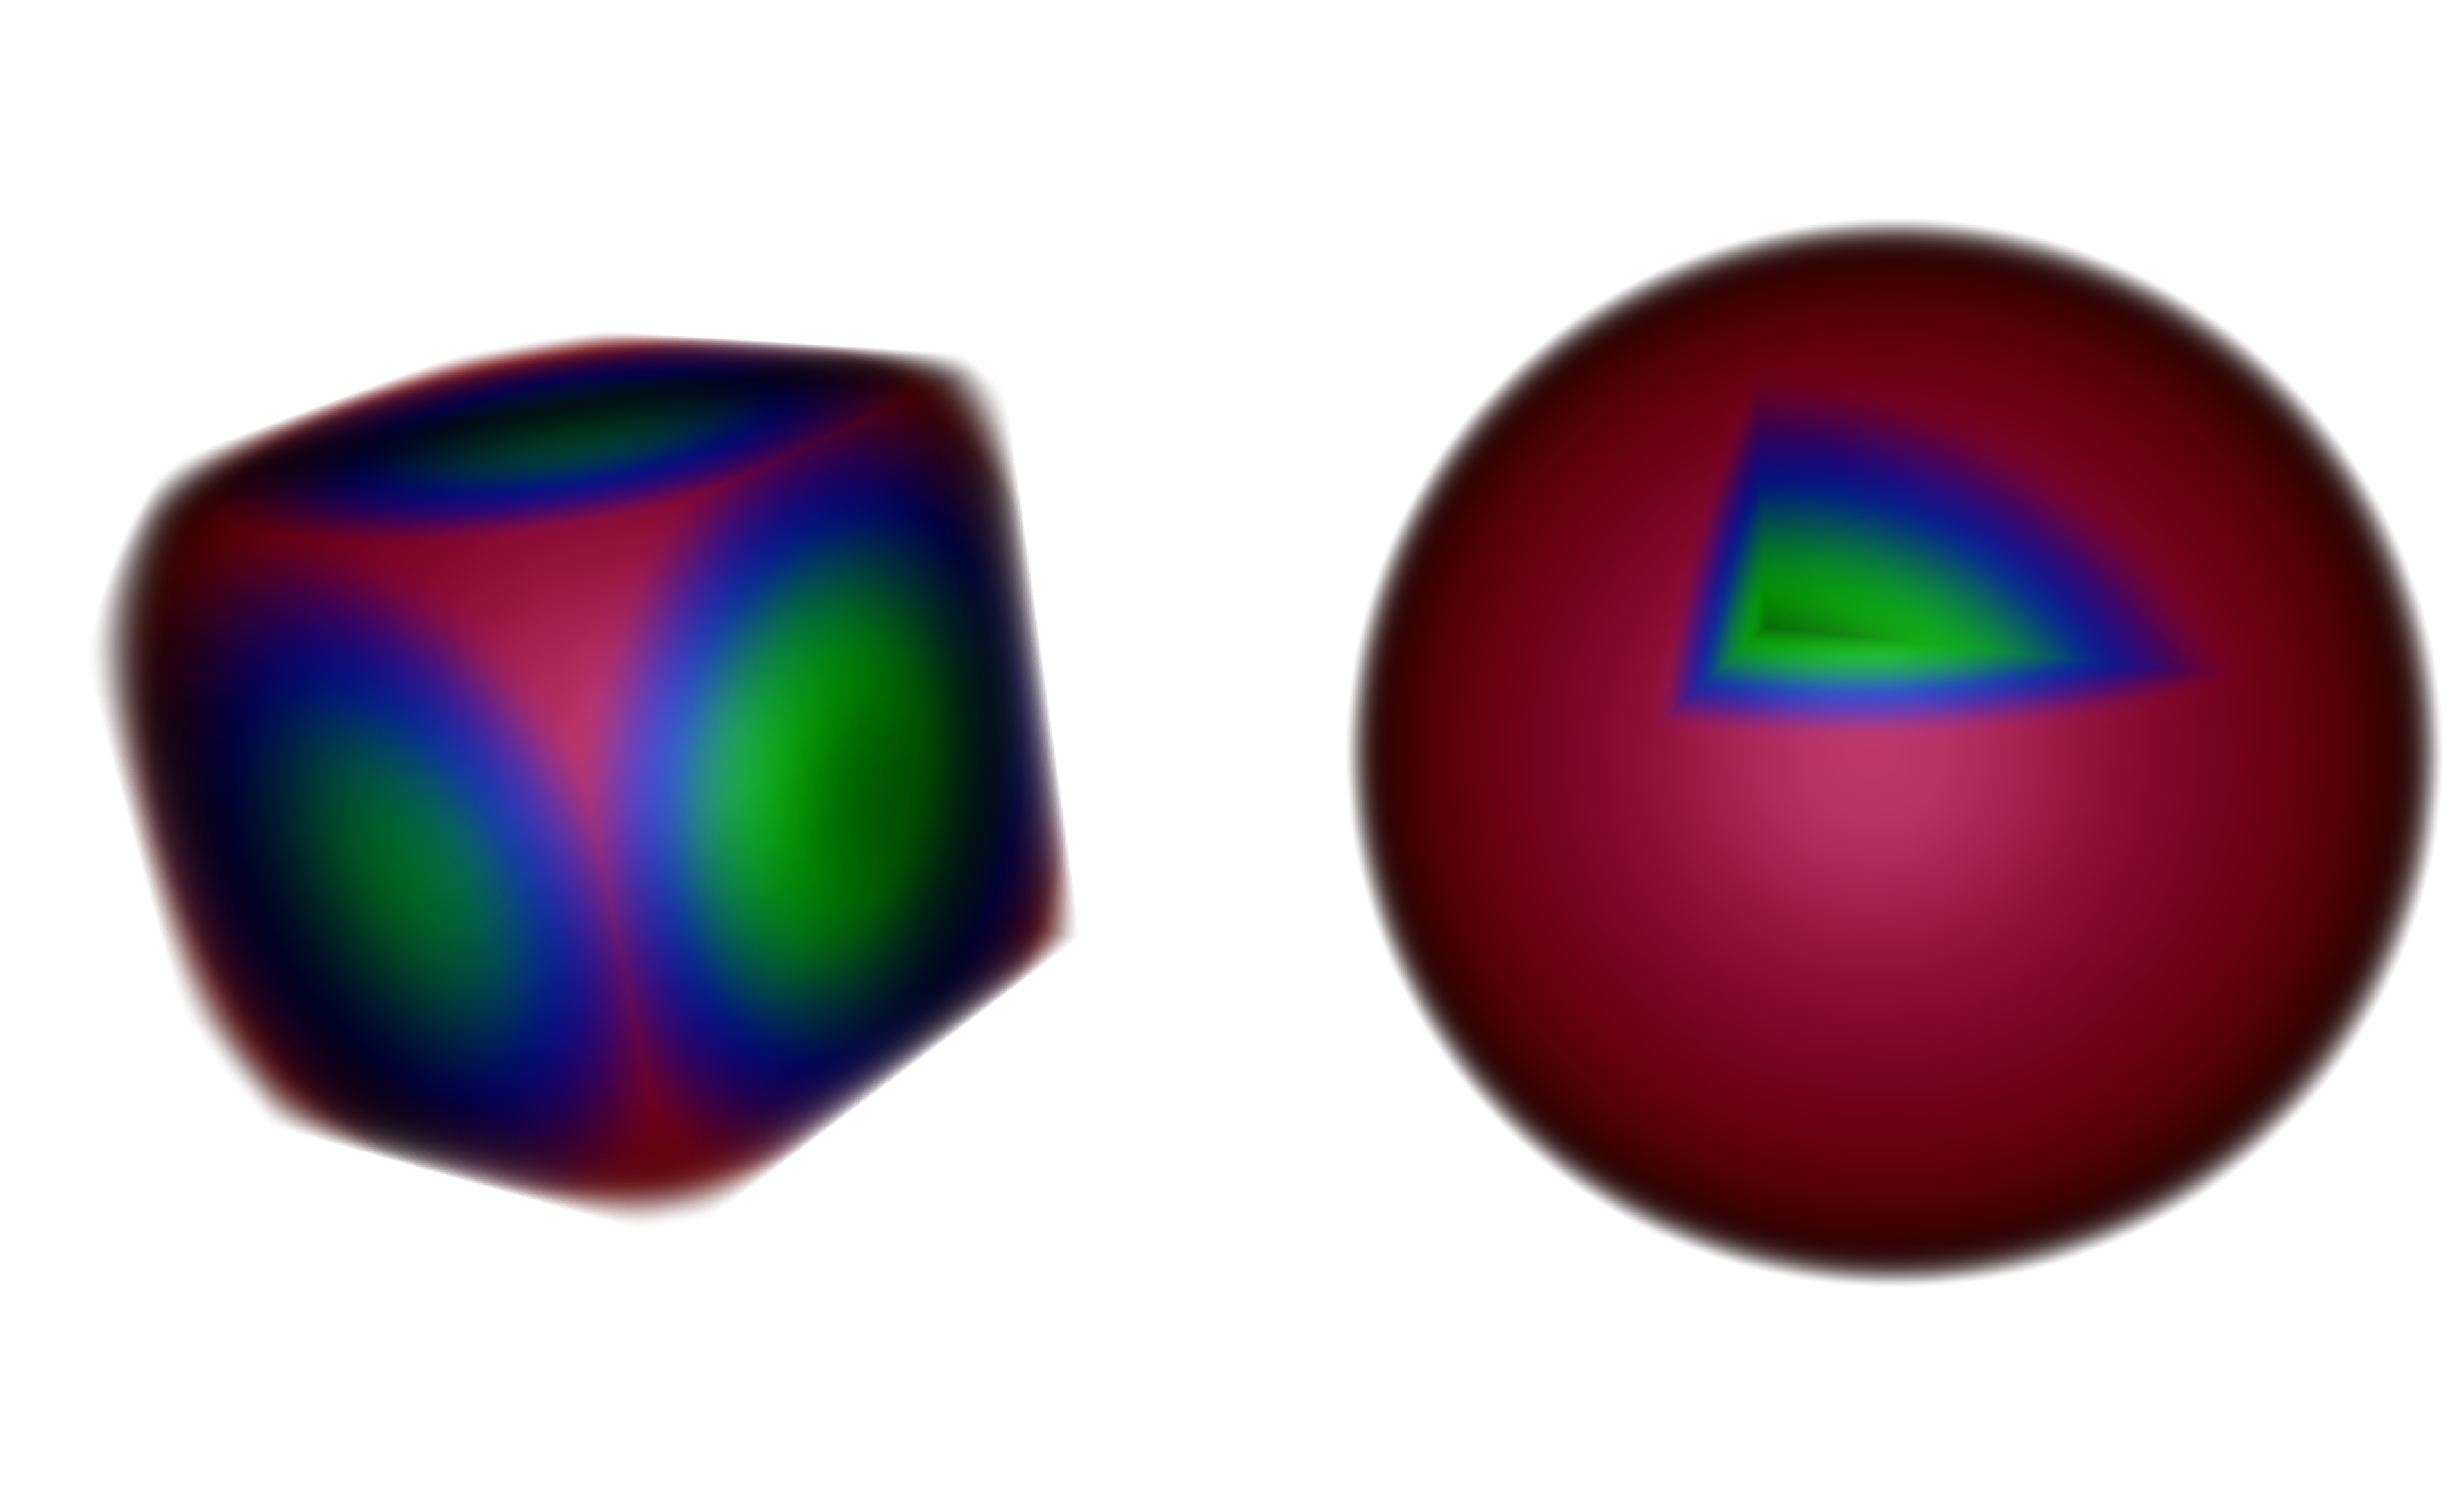
\includegraphics[width=2.5in]{SphereCropping.png}
%   \caption{A sphere is cropped using two different configurations of cropping regions.}
%   \label{fig:cropping}
% \end{figure}

\subsection{Broad Support of Data Types}
\label{data-types}
The mapper supports most signed and unsigned data types such as short, int,
float and double as well as the two most common data abstractions in VTK,
cell and point data.  Bias and scale factors are pre-computed and passed into
the fragment shader to normalize the data values for correct look-up table
mapping.

\begin{figure}[htb]
  \centering
  \begin{subfigure}[b]{.55\columnwidth}
    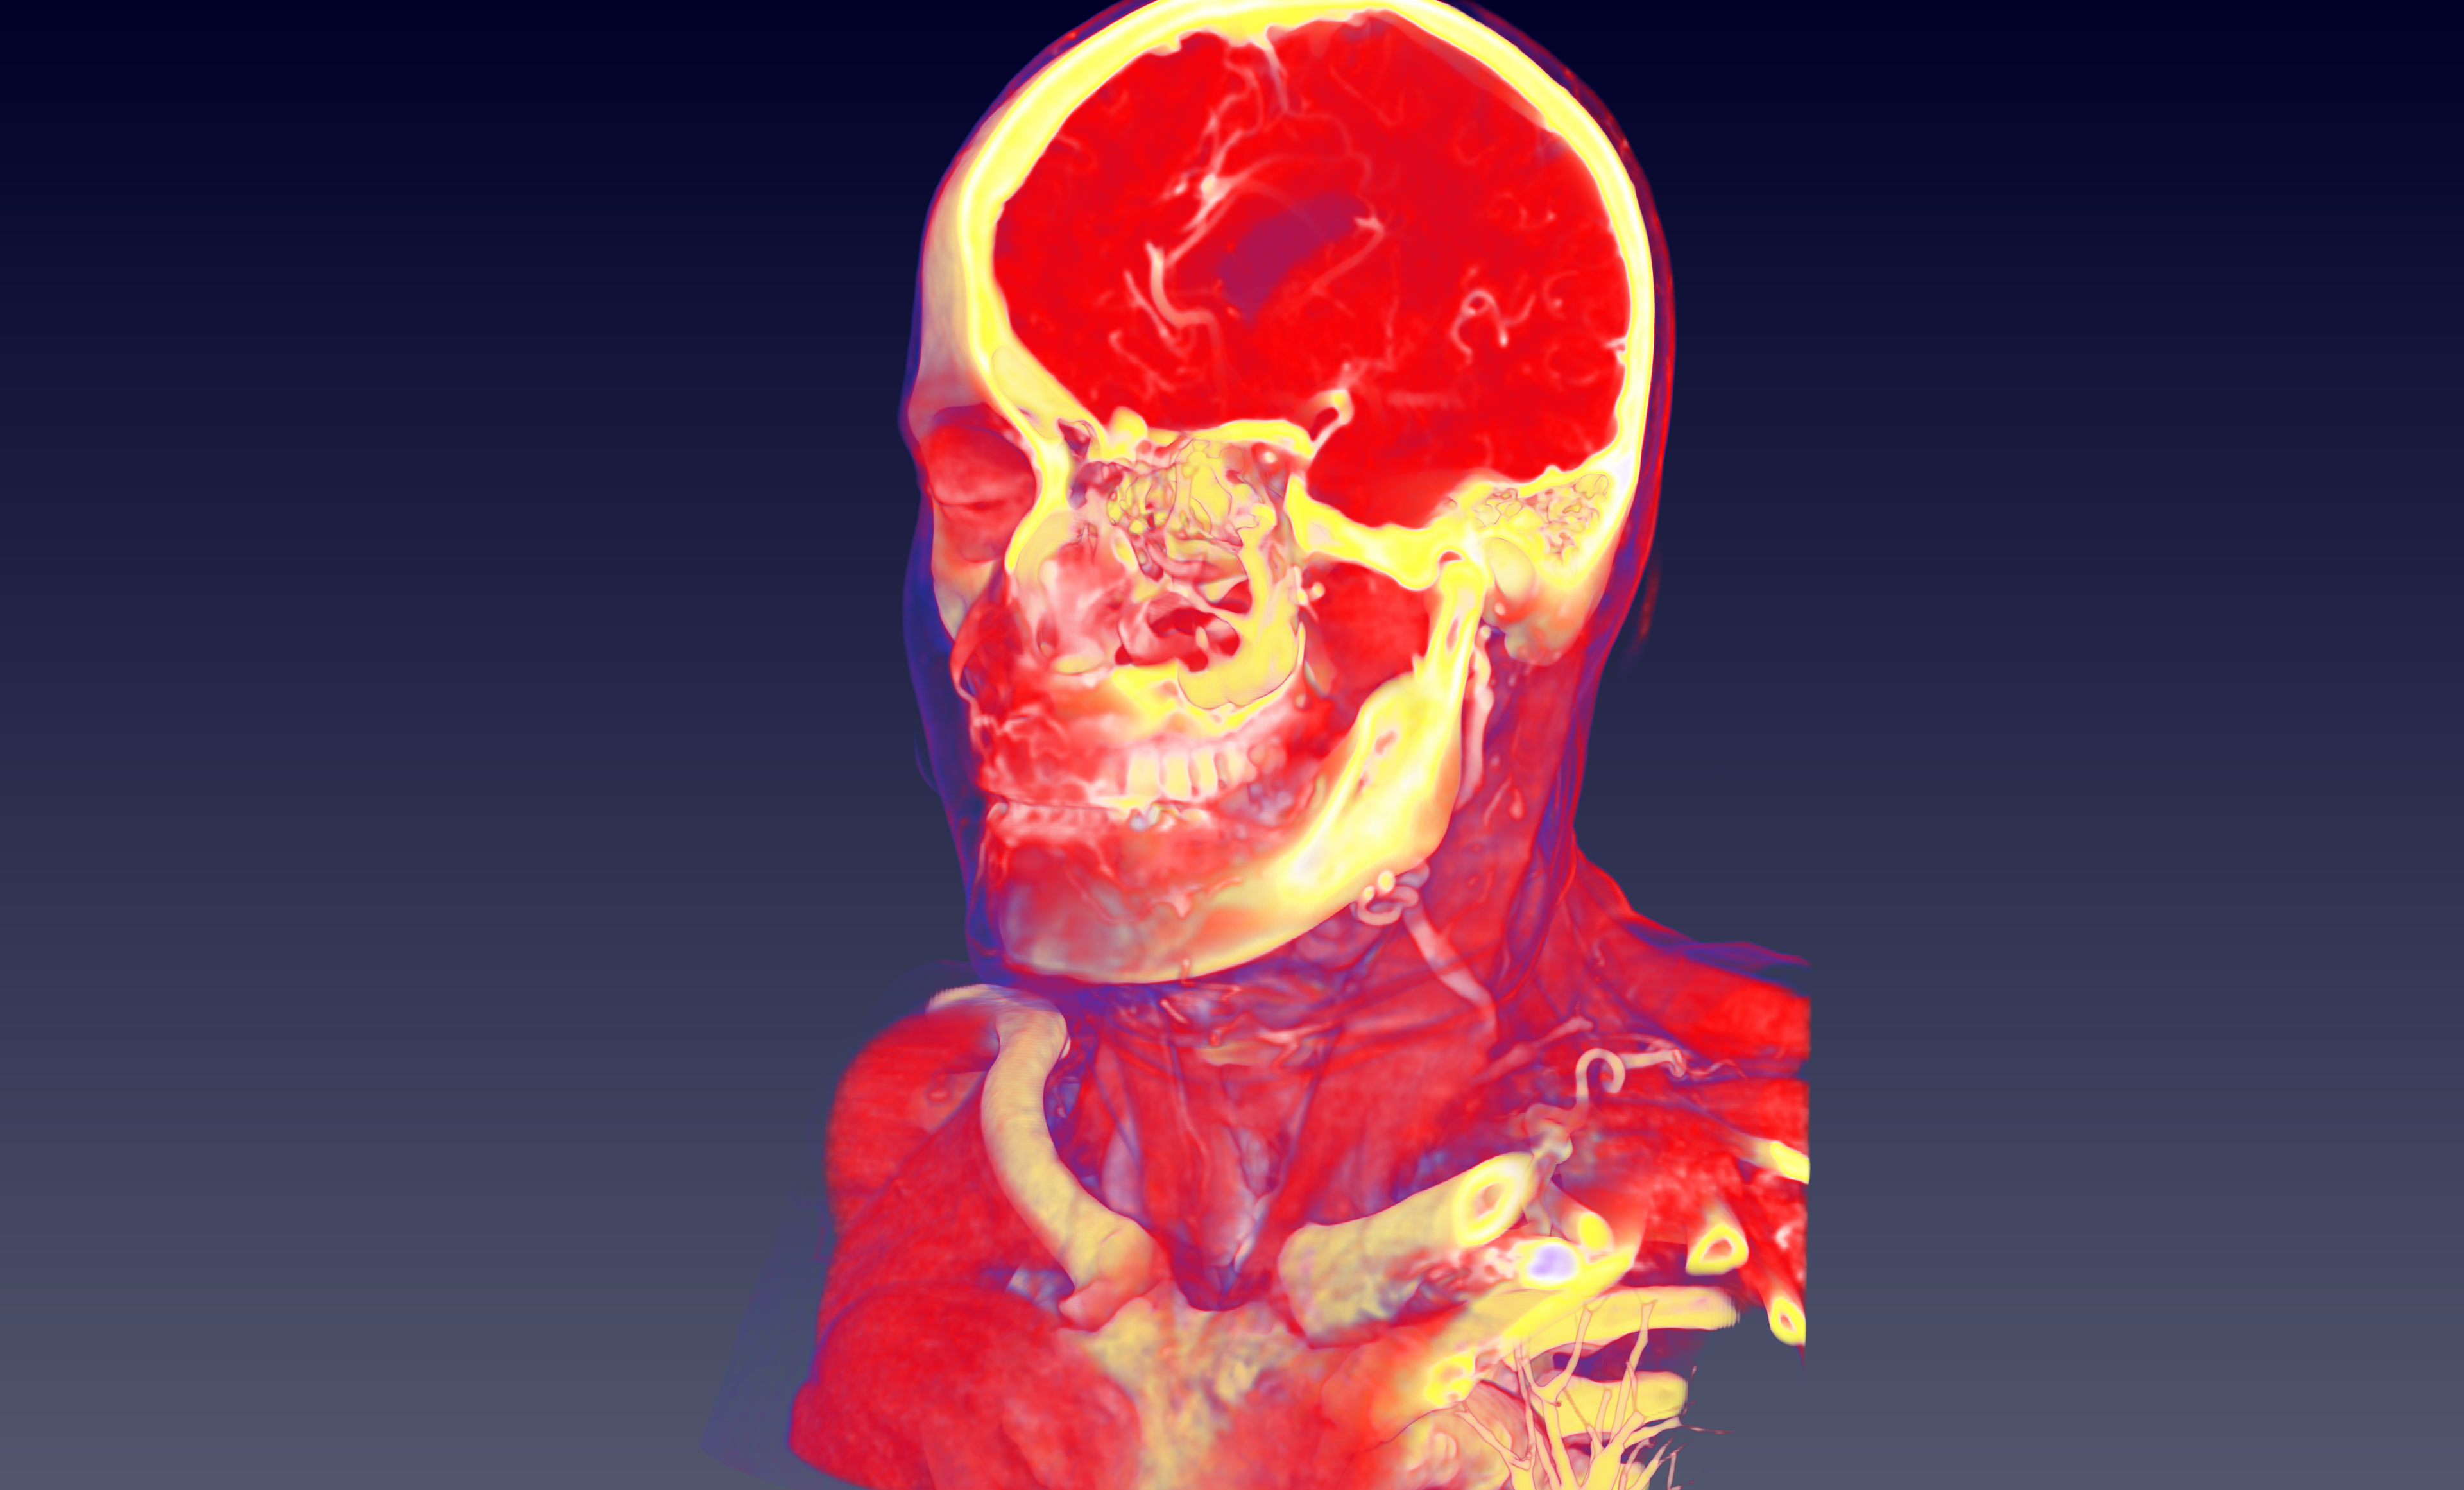
\includegraphics[width=\textwidth, height=7cm]{HeadClippingOblique}
    \caption{Oblique clipping plane}
    \label{fig:clipoblique}
  \end{subfigure}%
  \hspace*{\fill}
  \begin{subfigure}[b]{.43\columnwidth}
    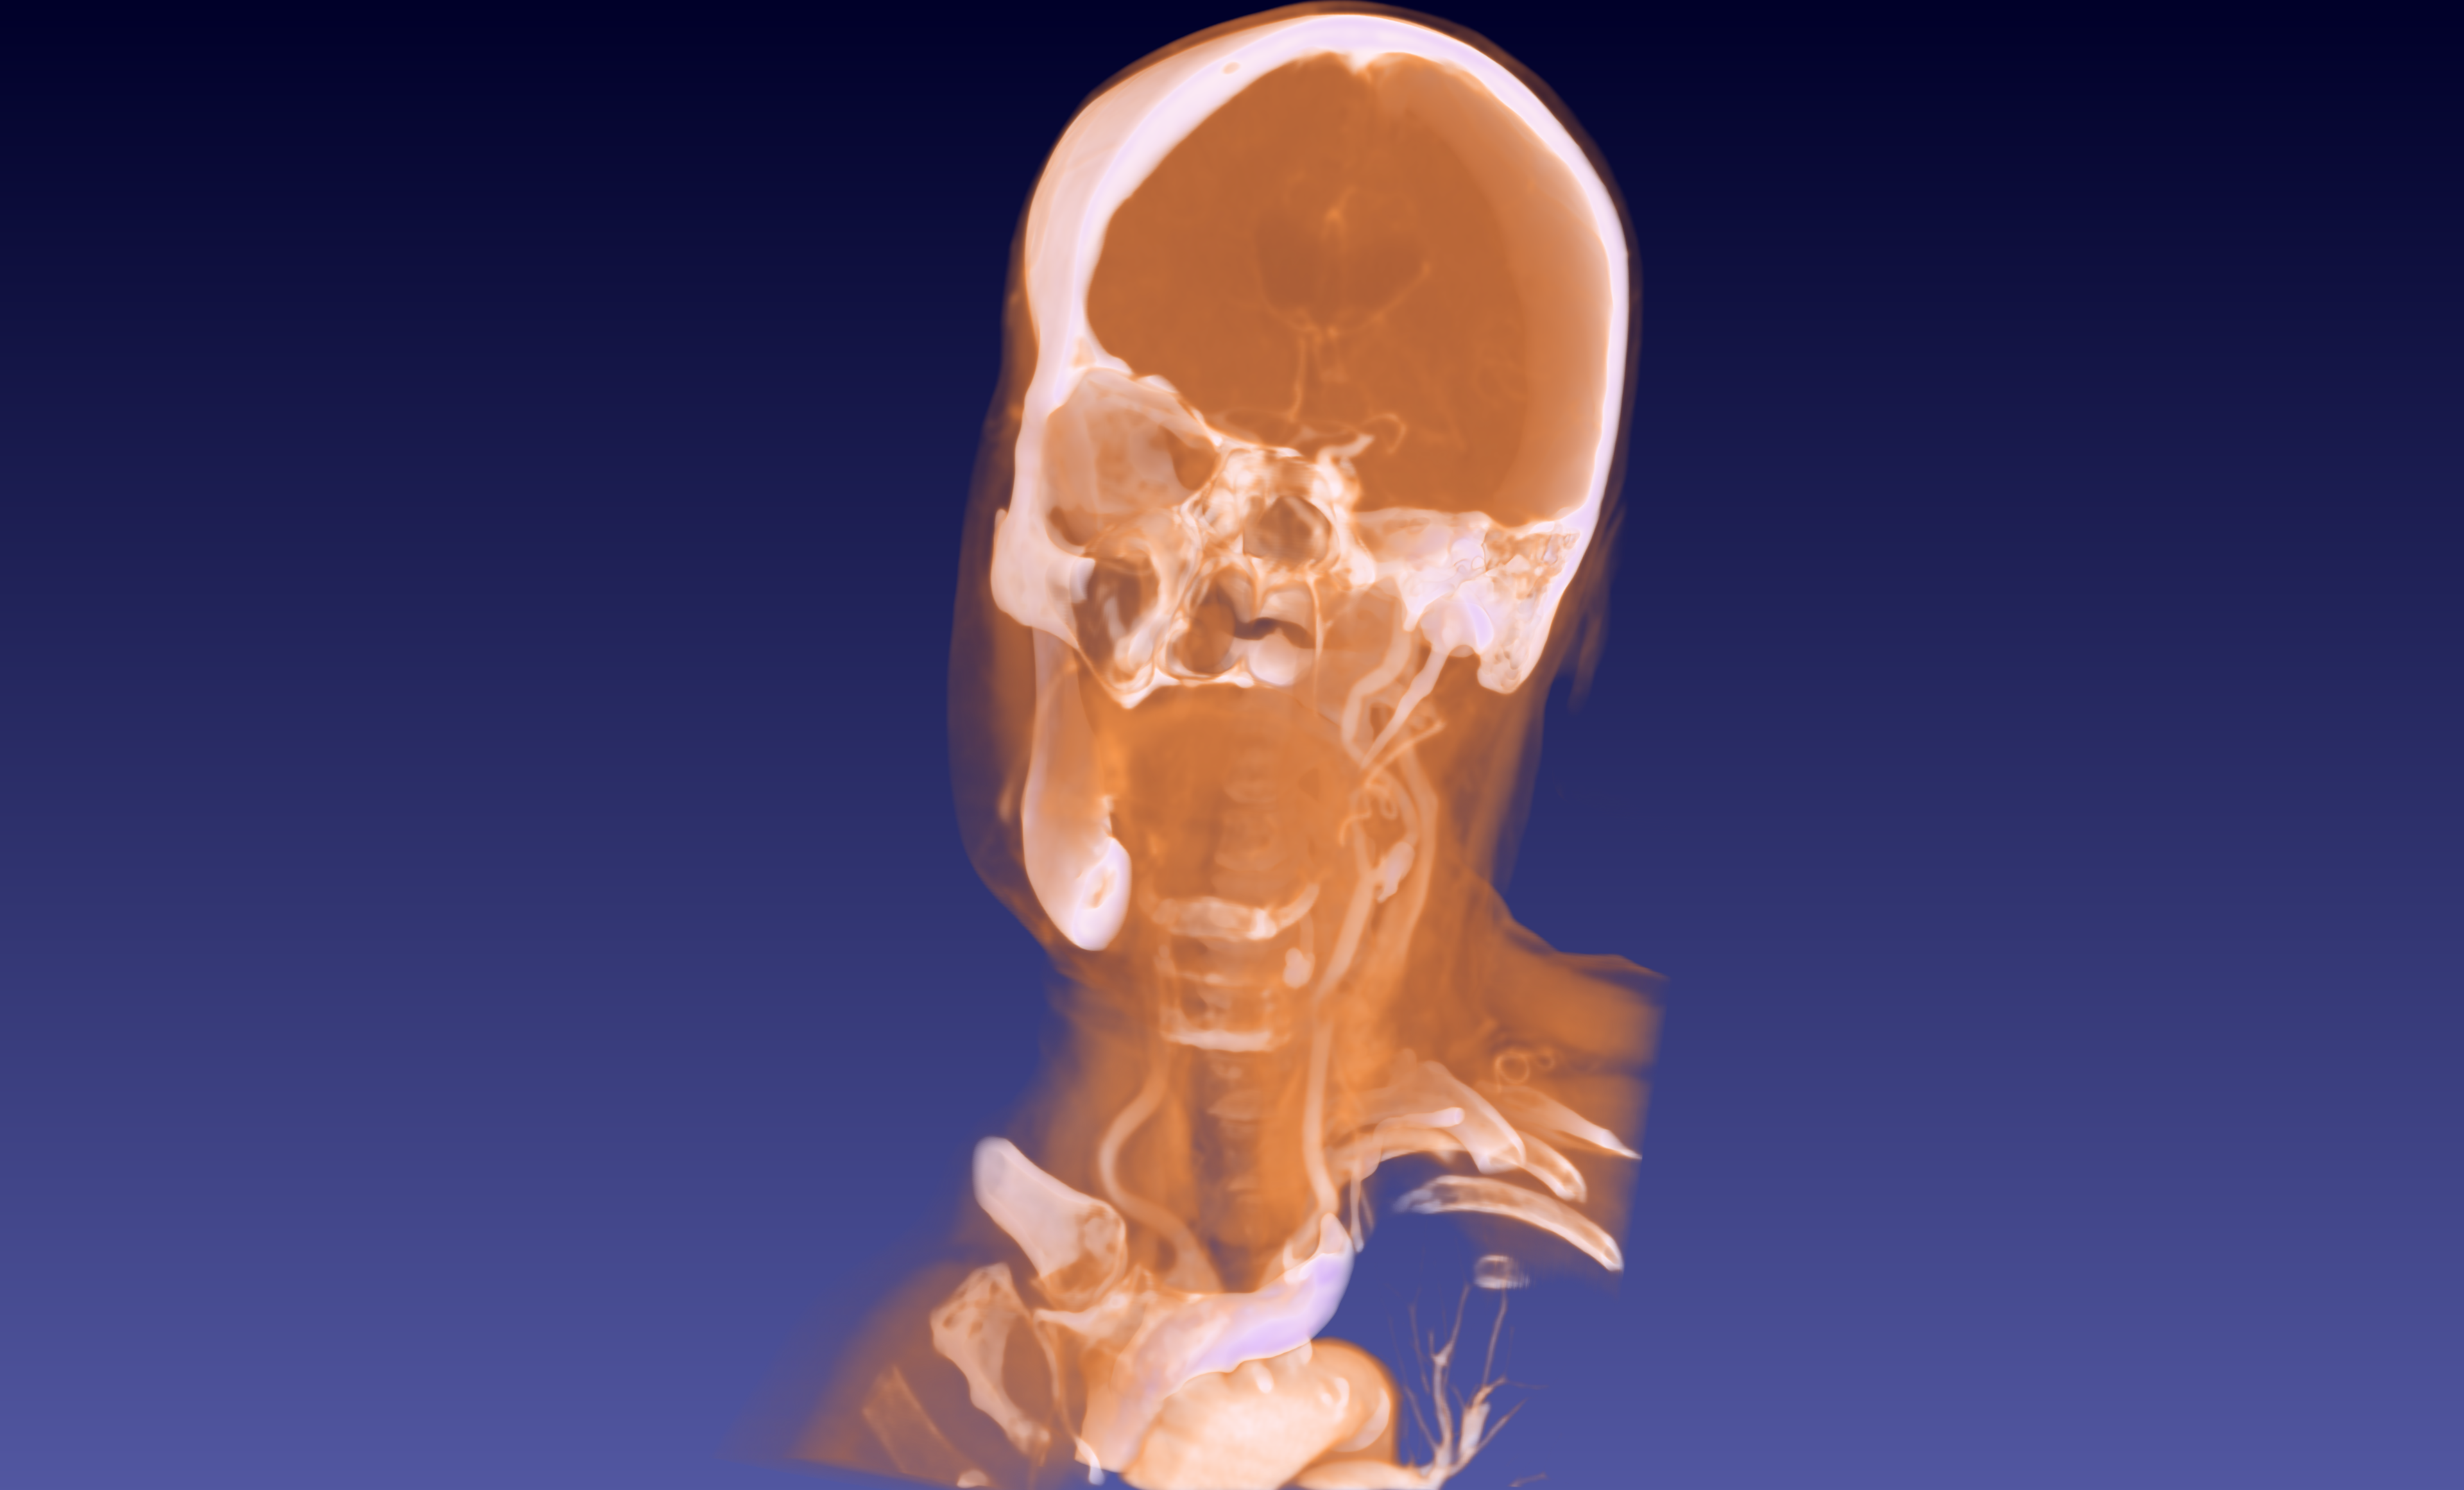
\includegraphics[width=\textwidth, height=3.19cm]{HeadClippingSlabNoShading}
    \caption{Without shading}
    \label{fig:clipnoshading}
    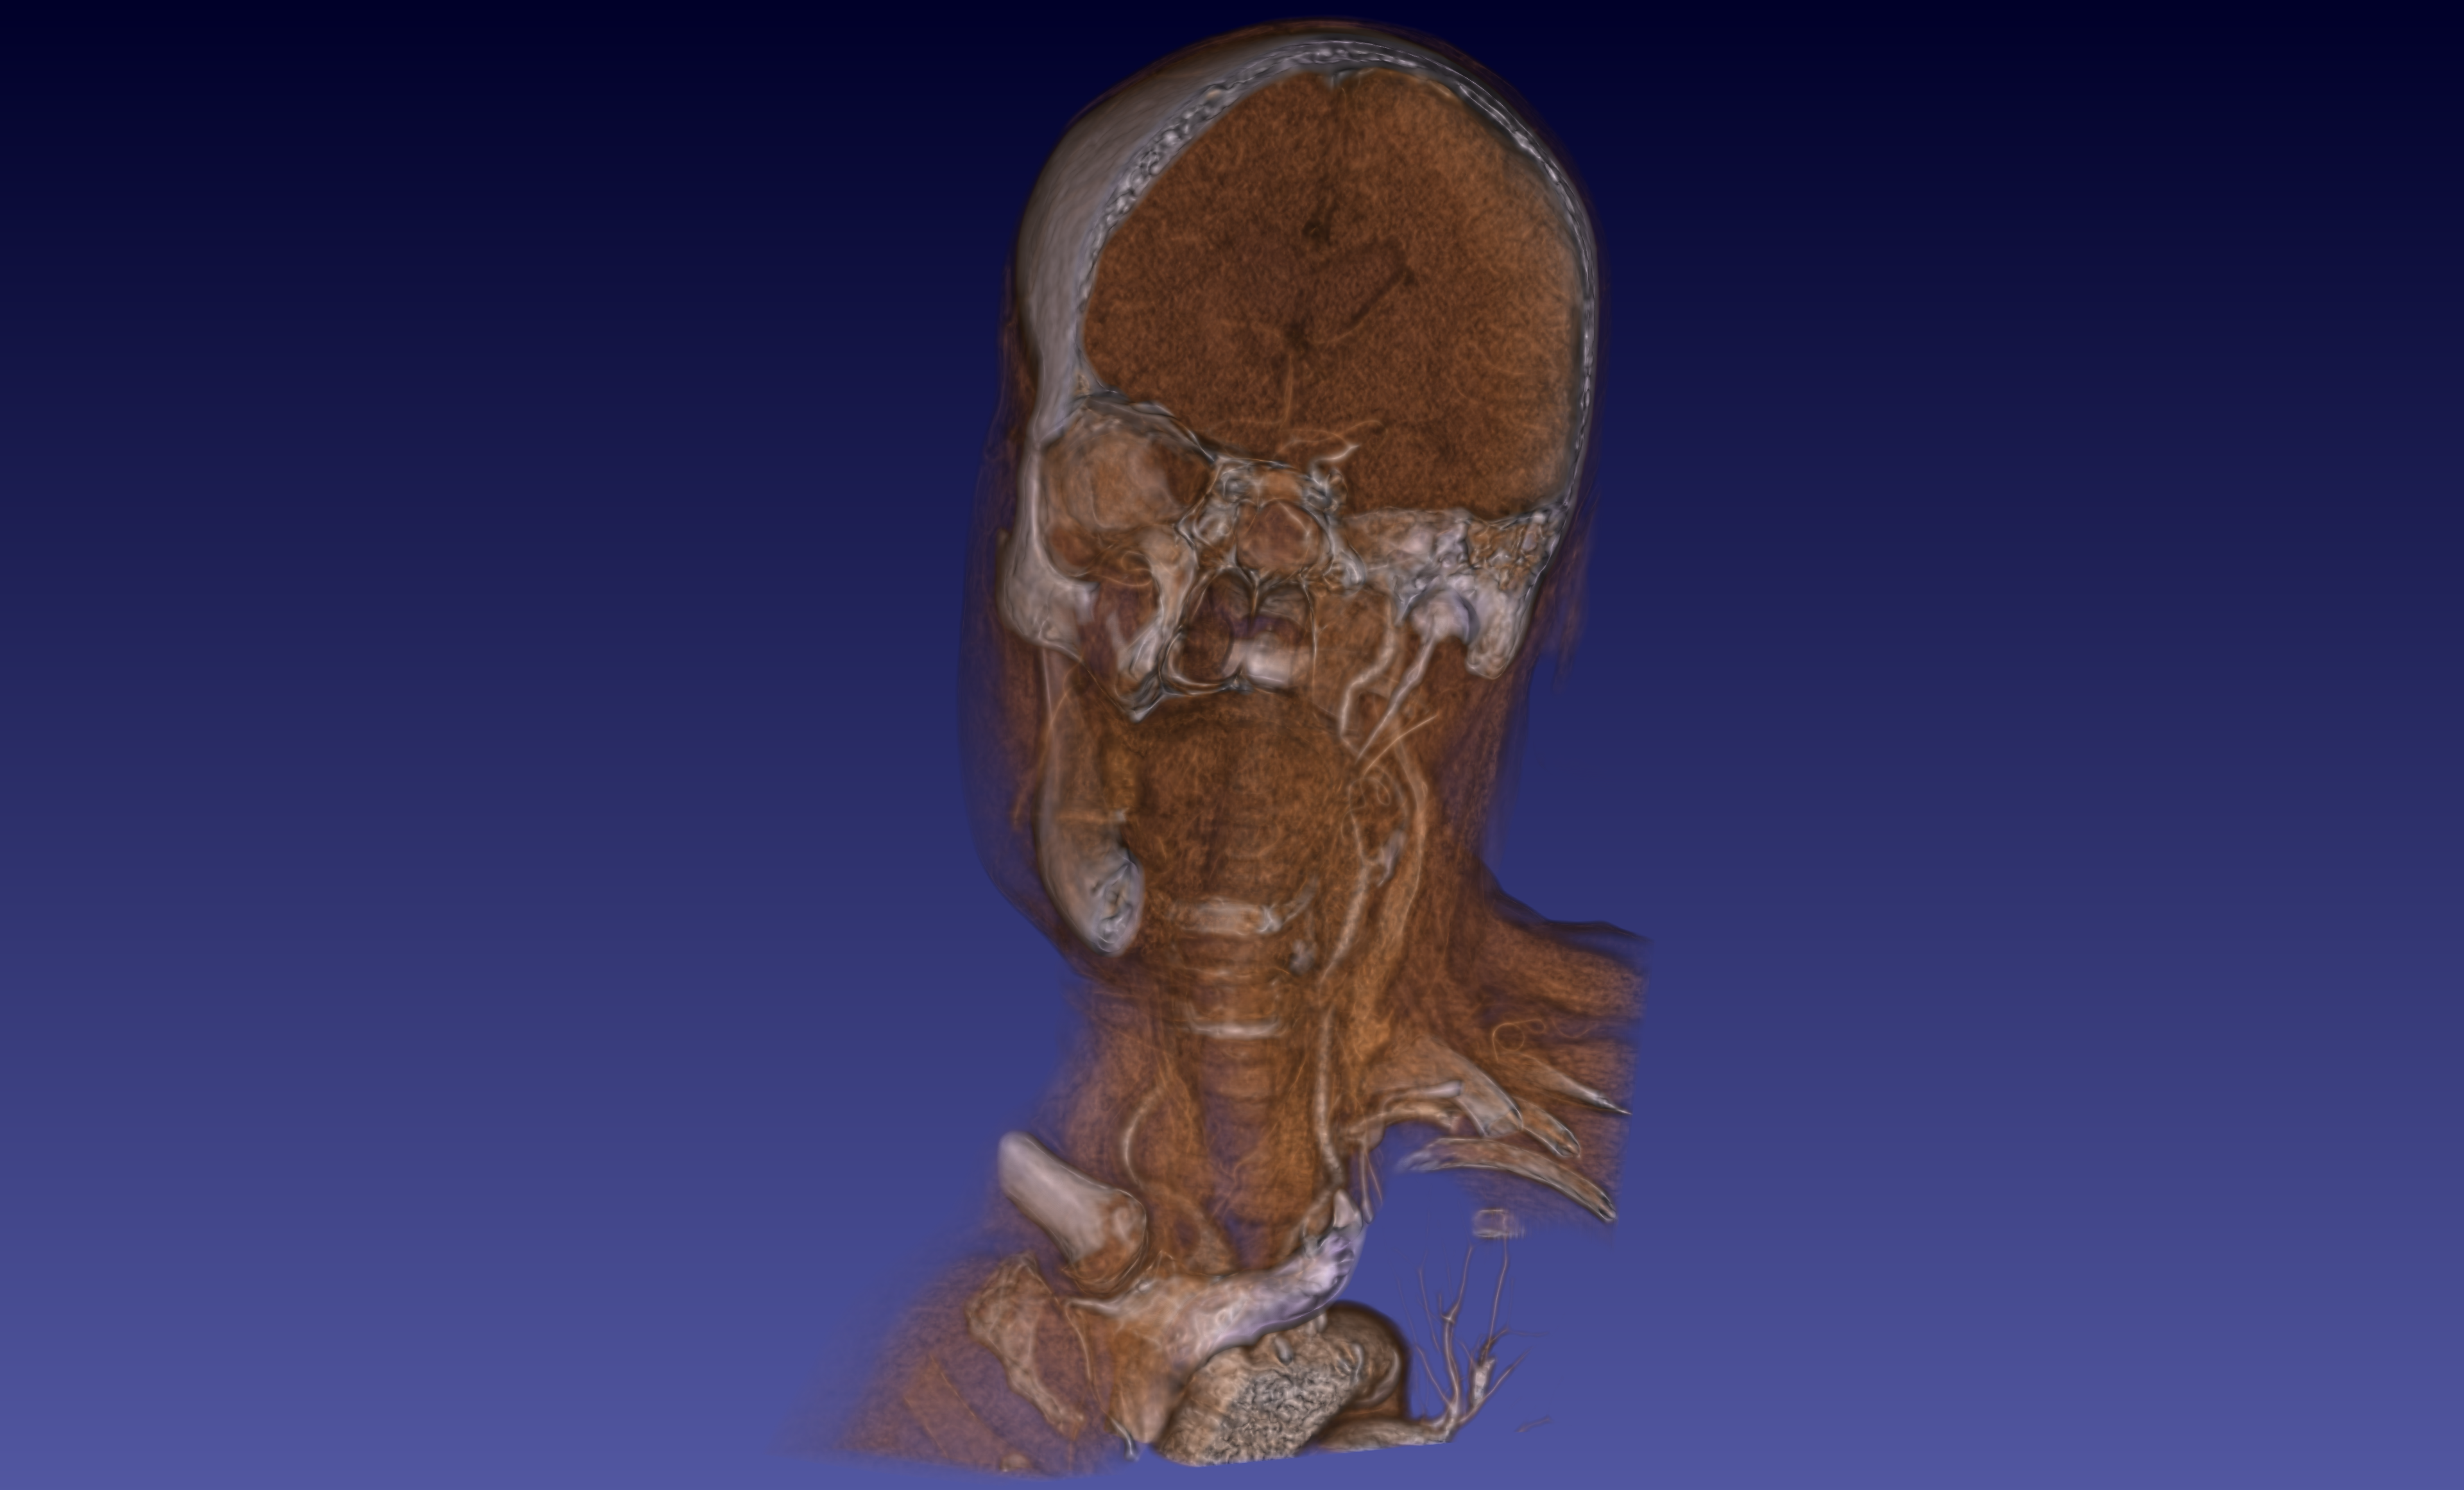
\includegraphics[width=\textwidth, height=3.19cm]{HeadClippingSlabShading}
    \caption{With shading}
    \label{fig:clipshading}
  \end{subfigure}
  %\begin{subfigure}[b]{.5\columnwidth}
    %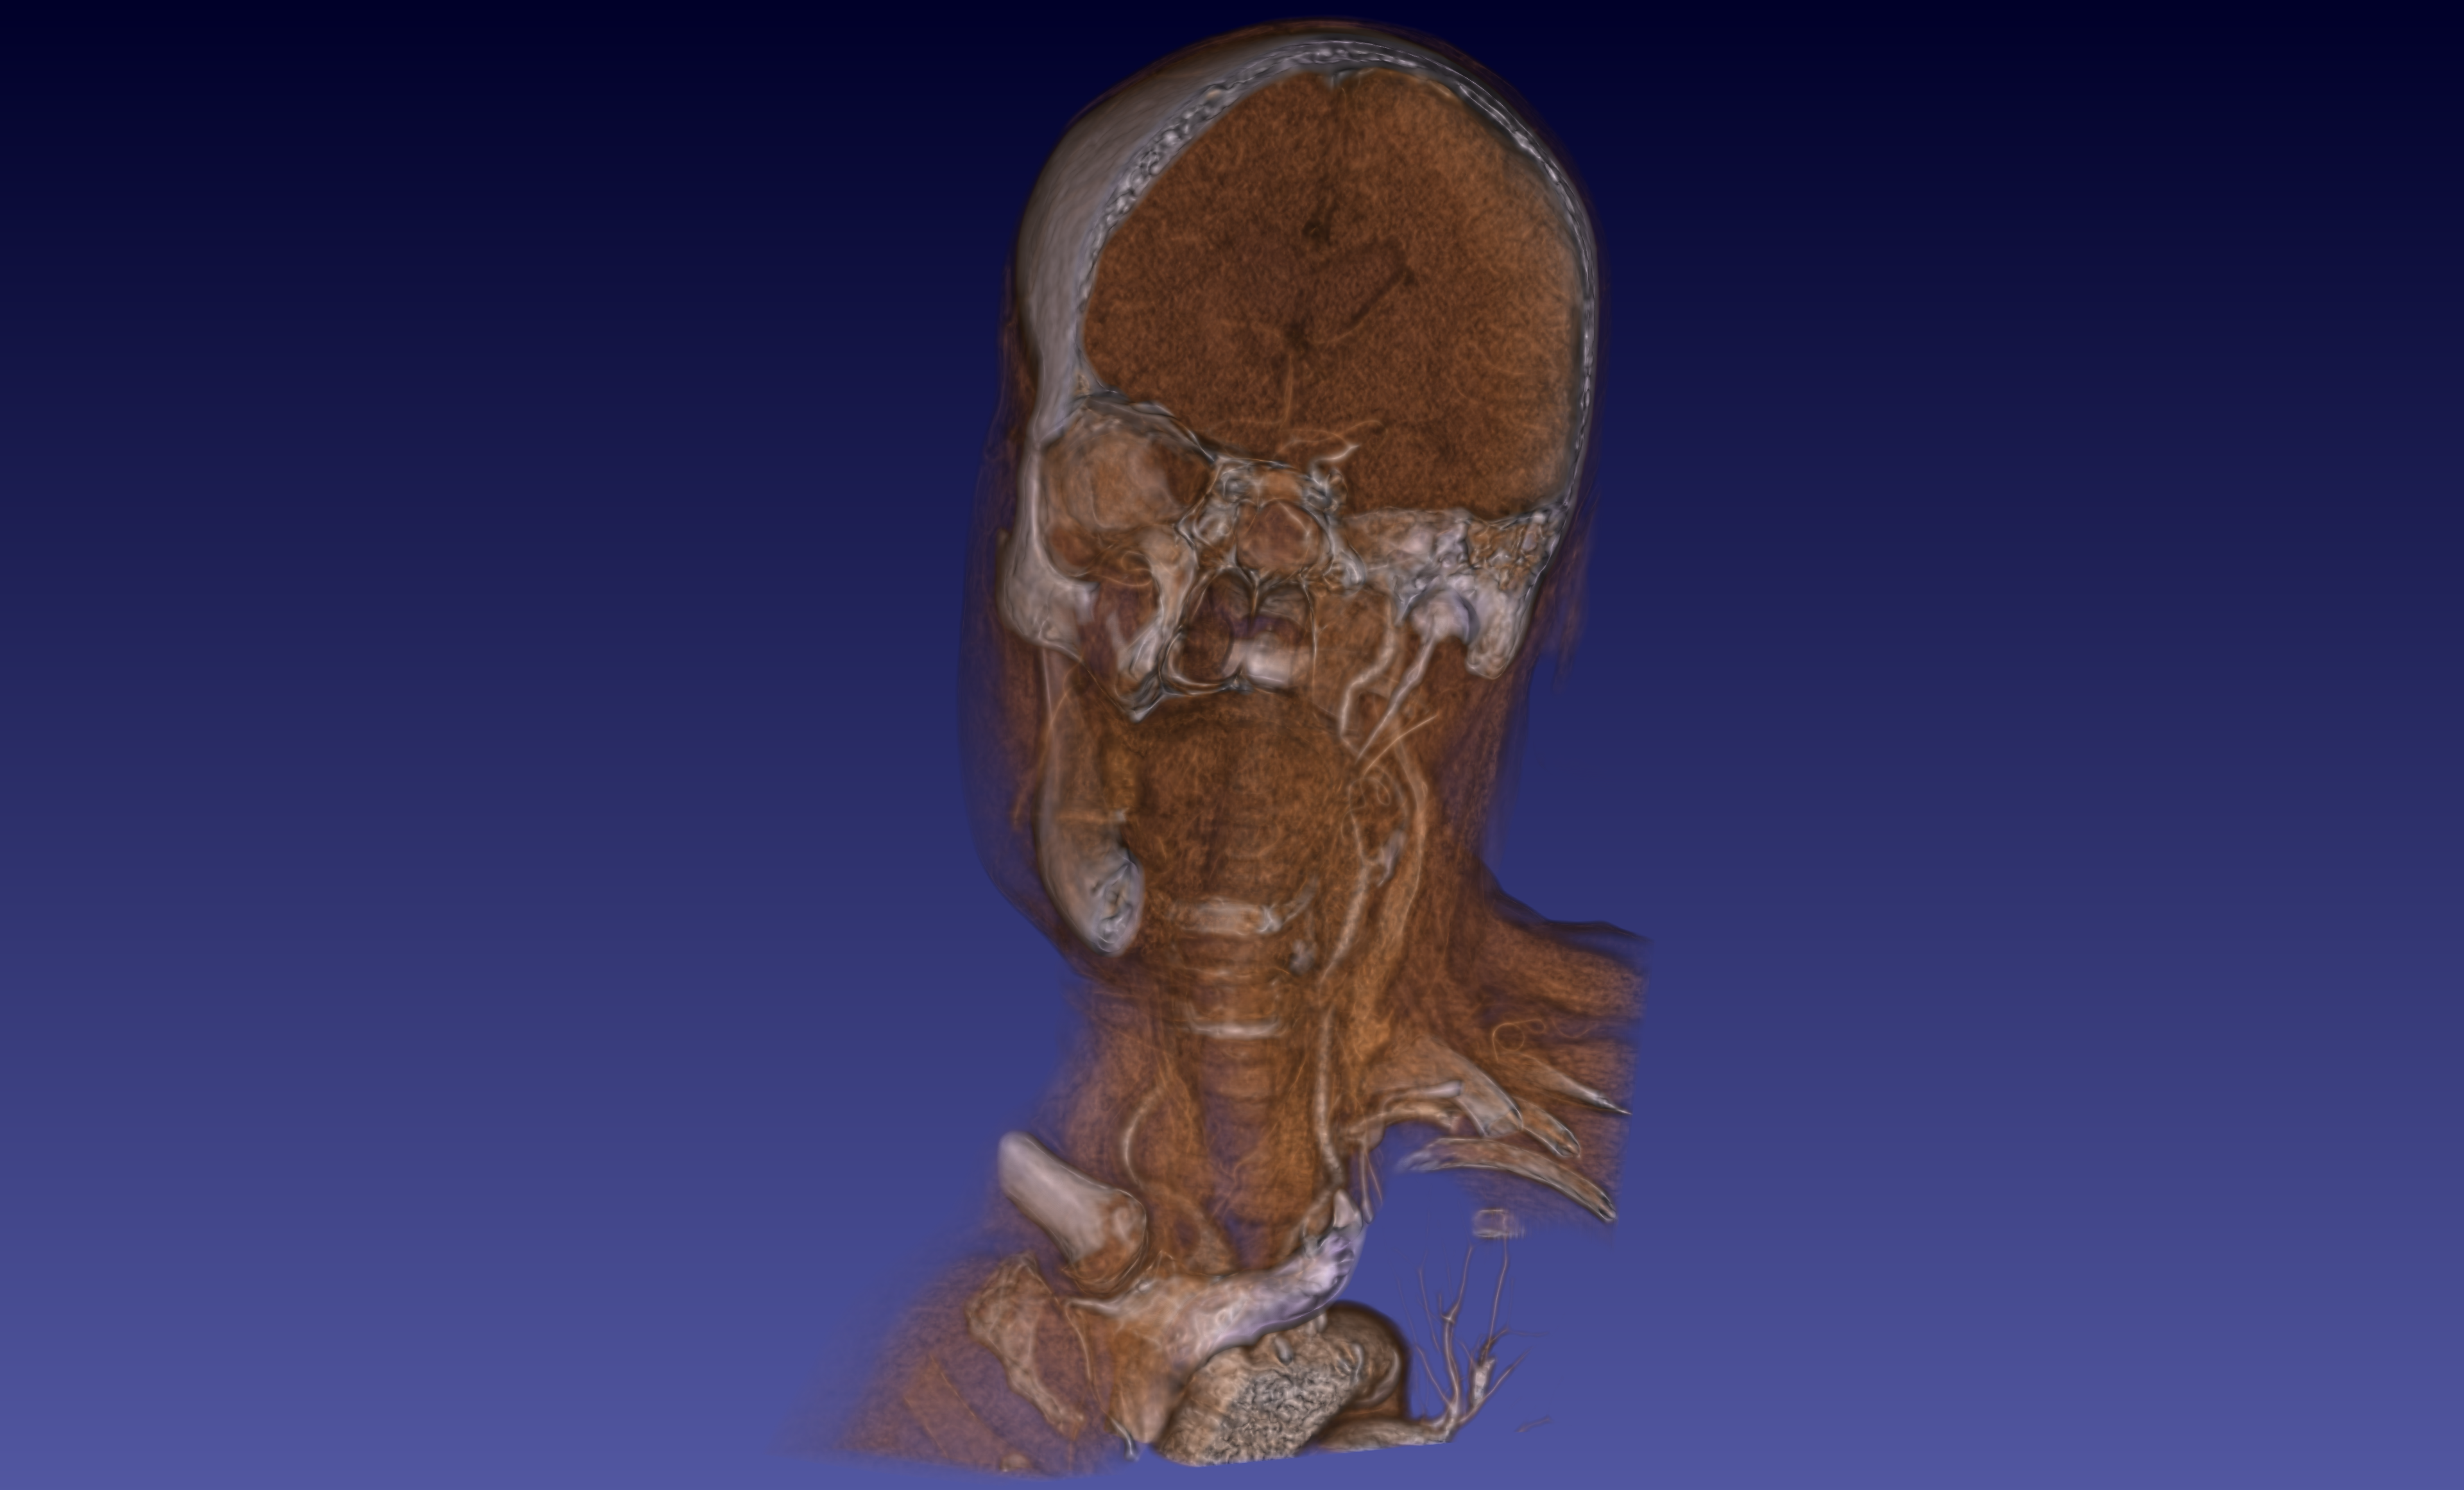
\includegraphics[width=\textwidth, height=3cm]{HeadClippingSlabShading}
    %\caption{With shading}
    %\label{fig:clipshading}
  %\end{subfigure}

  \caption{Clipping planes with~\texttt{vtkGPUVolumeRayCastMapper}. Example of
    an oblique~(a) i.e. off-axis clipping plane through the volume.
    A clipping plane through the volume without~(b) and with~(c)
    surface shading.}
  \label{fig:clipping}
\end{figure}

\subsection{Blending Modes}
\label{blending-modes}
The mapper supports composite blending, minimum intensity projection, maximum
intensity projection, additive intensity and average intensity blending.  These
blending modes are useful for the variety of use case found in medical
computing.  The most common one, which is also the default, is the composite
blending mode.  See~\Autoref{fig:blendingmodes} for an example of the different
blend modes on the same data.

\begin{figure}[htb]
  \centering%
  \begin{subfigure}{.5\columnwidth}
    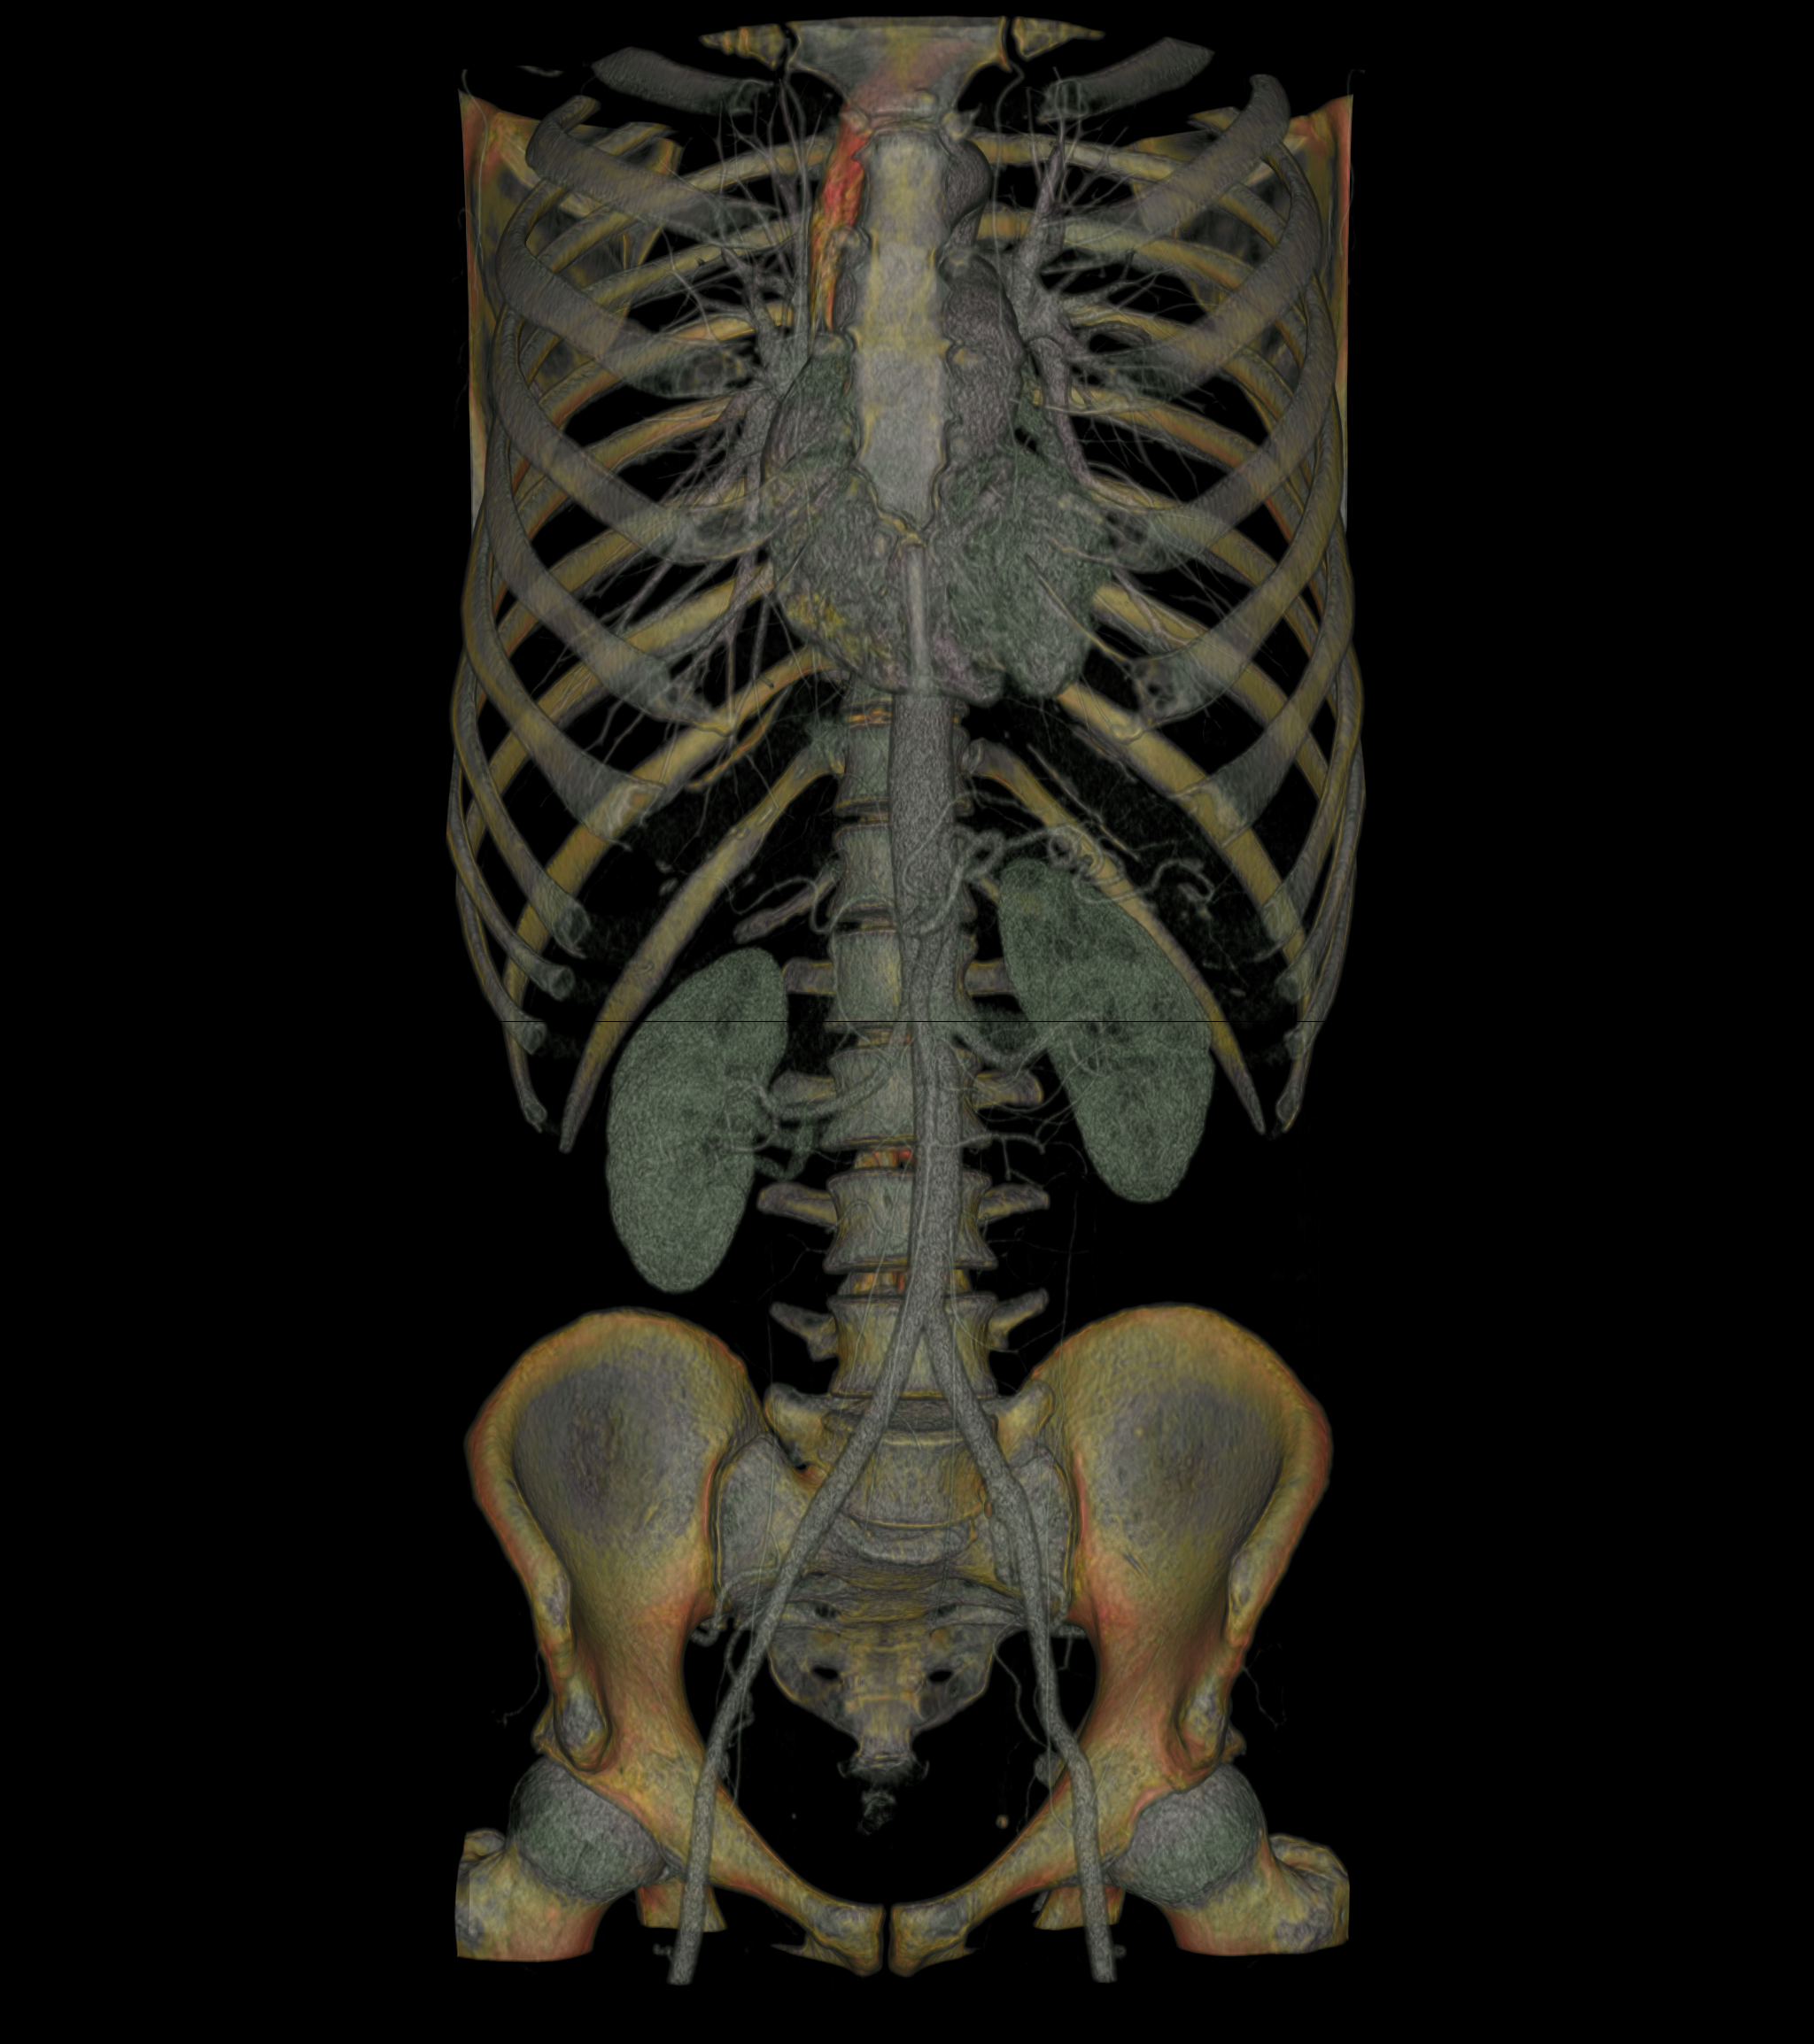
\includegraphics[width=\columnwidth]{TorsoBlendingComposite}
    \caption{Composite}
    \label{fig:blendcomposite}
  \end{subfigure}%
  \begin{subfigure}{.5\columnwidth}
    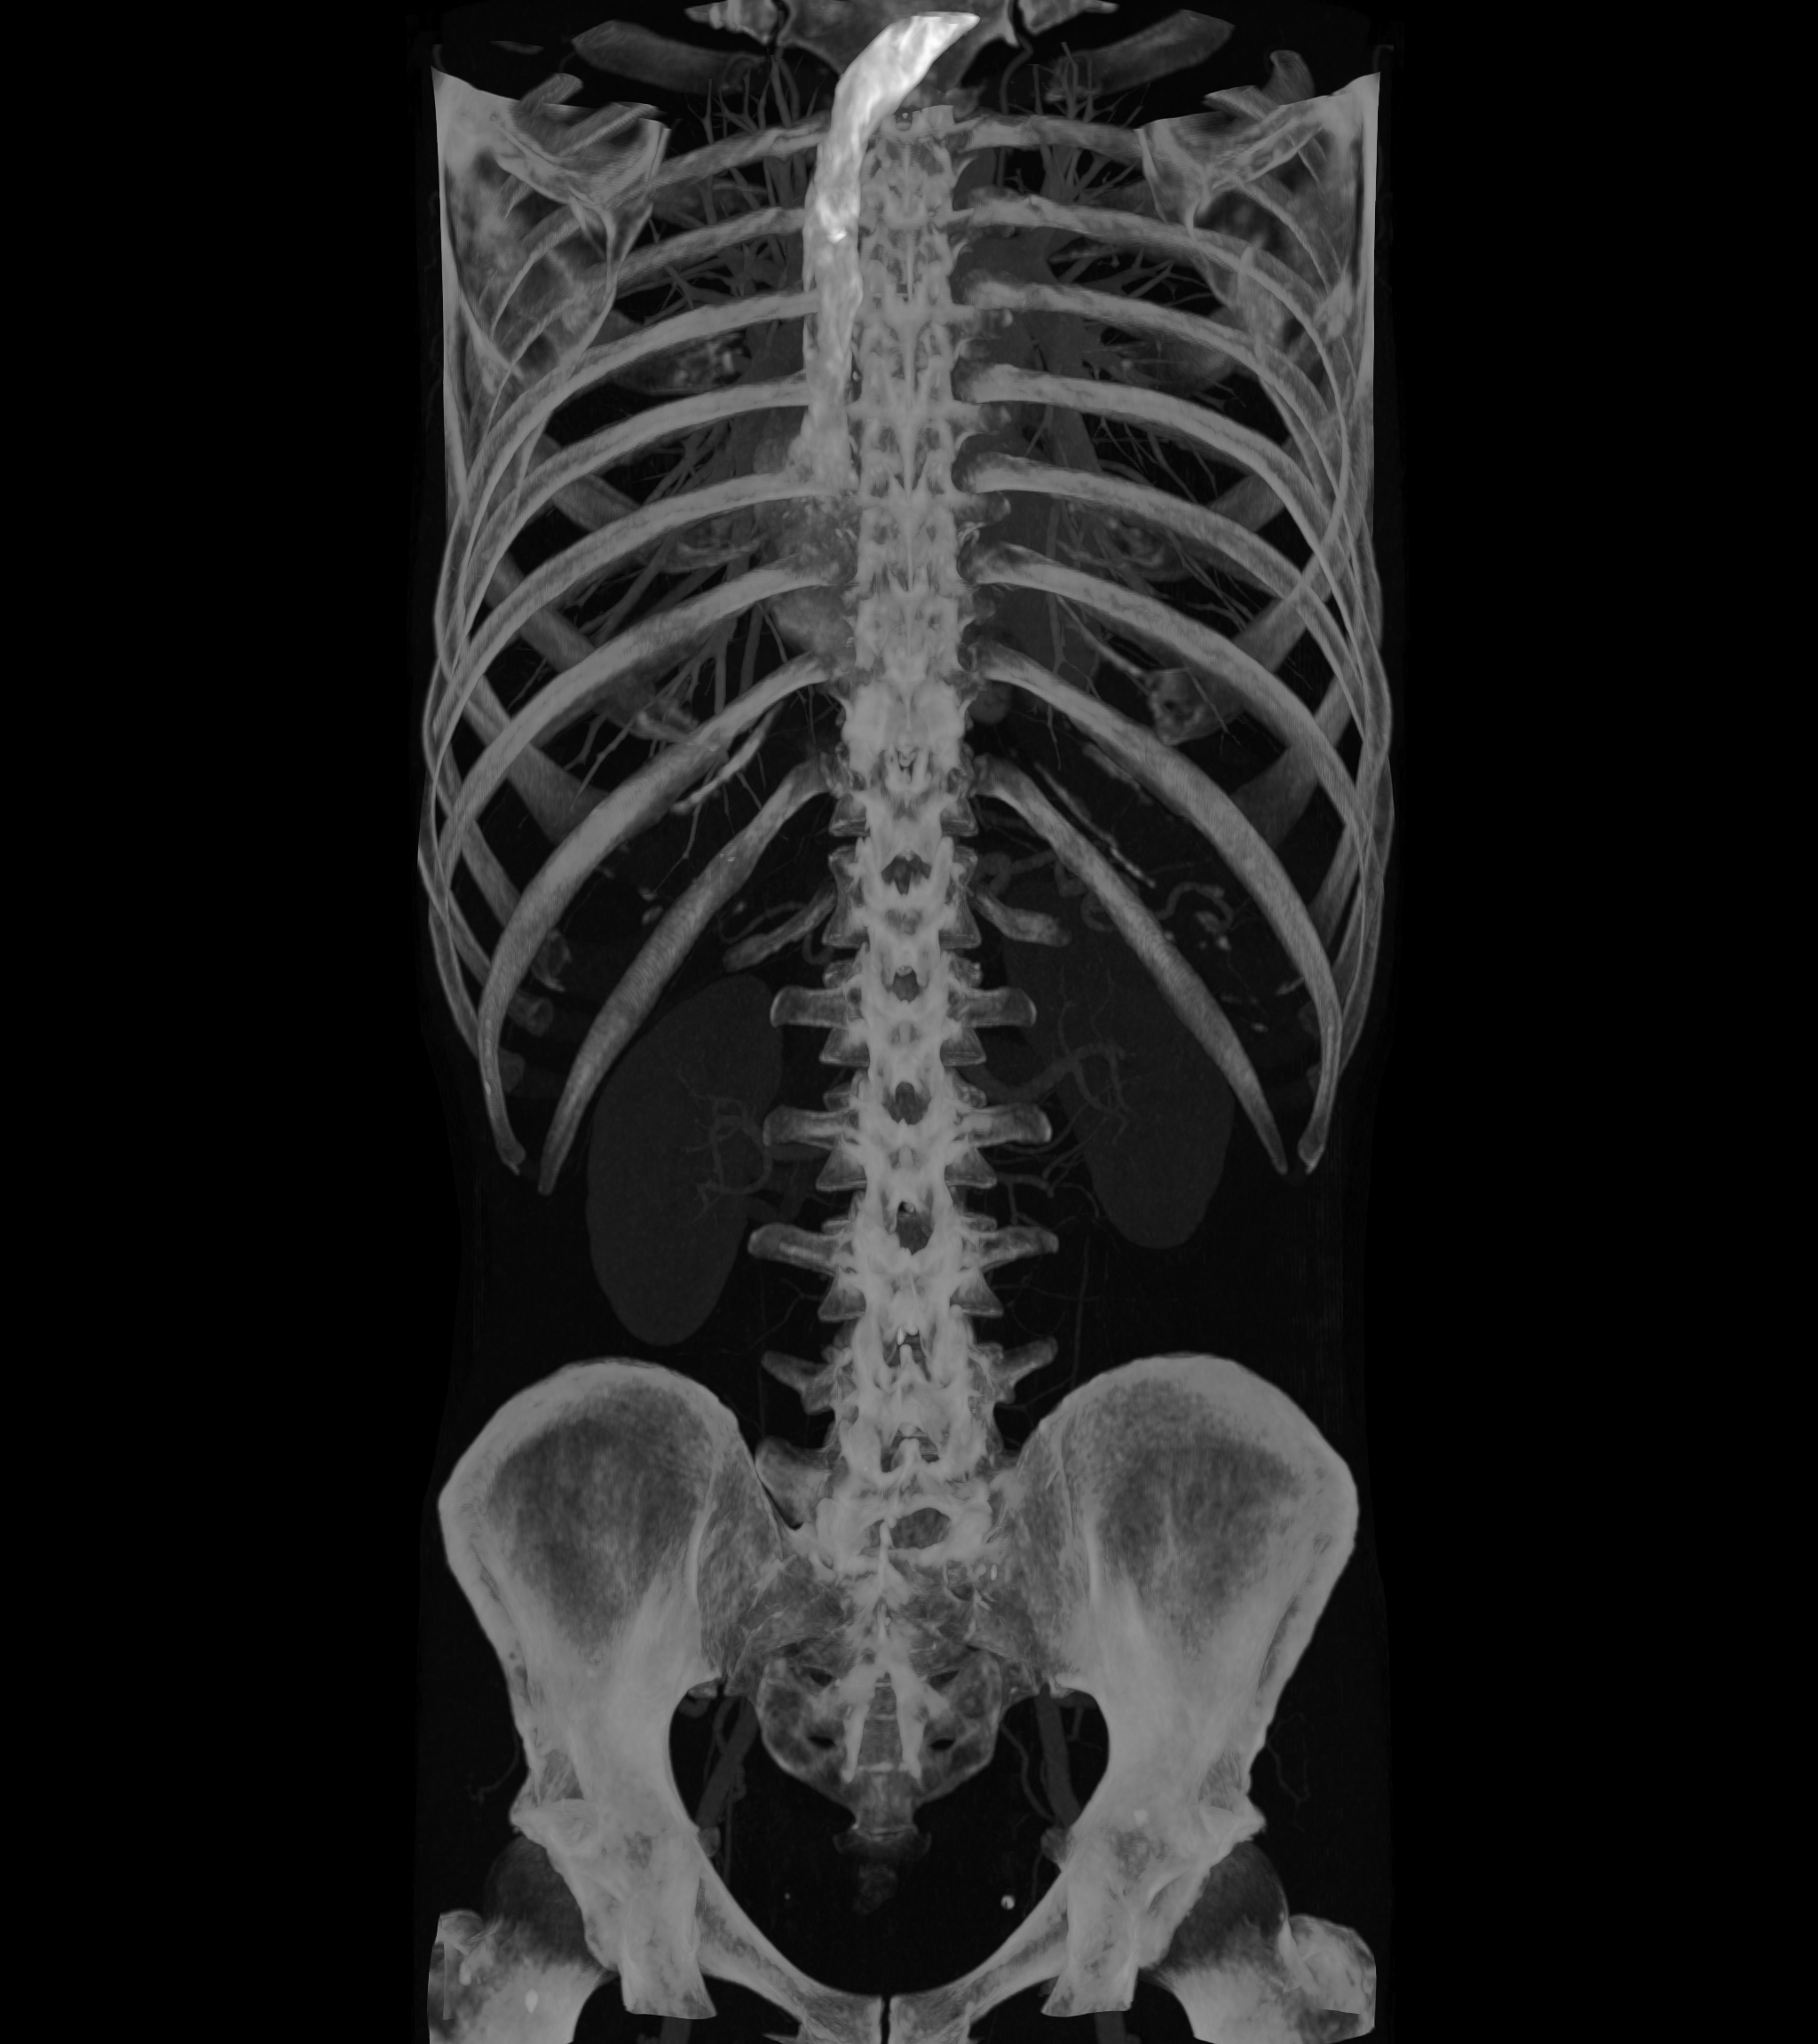
\includegraphics[width=\columnwidth]{TorsoBlendingMIP}
    \caption{Maximum Intensity}
    \label{fig:blendmax}
  \end{subfigure}
  \begin{subfigure}{.5\columnwidth}
    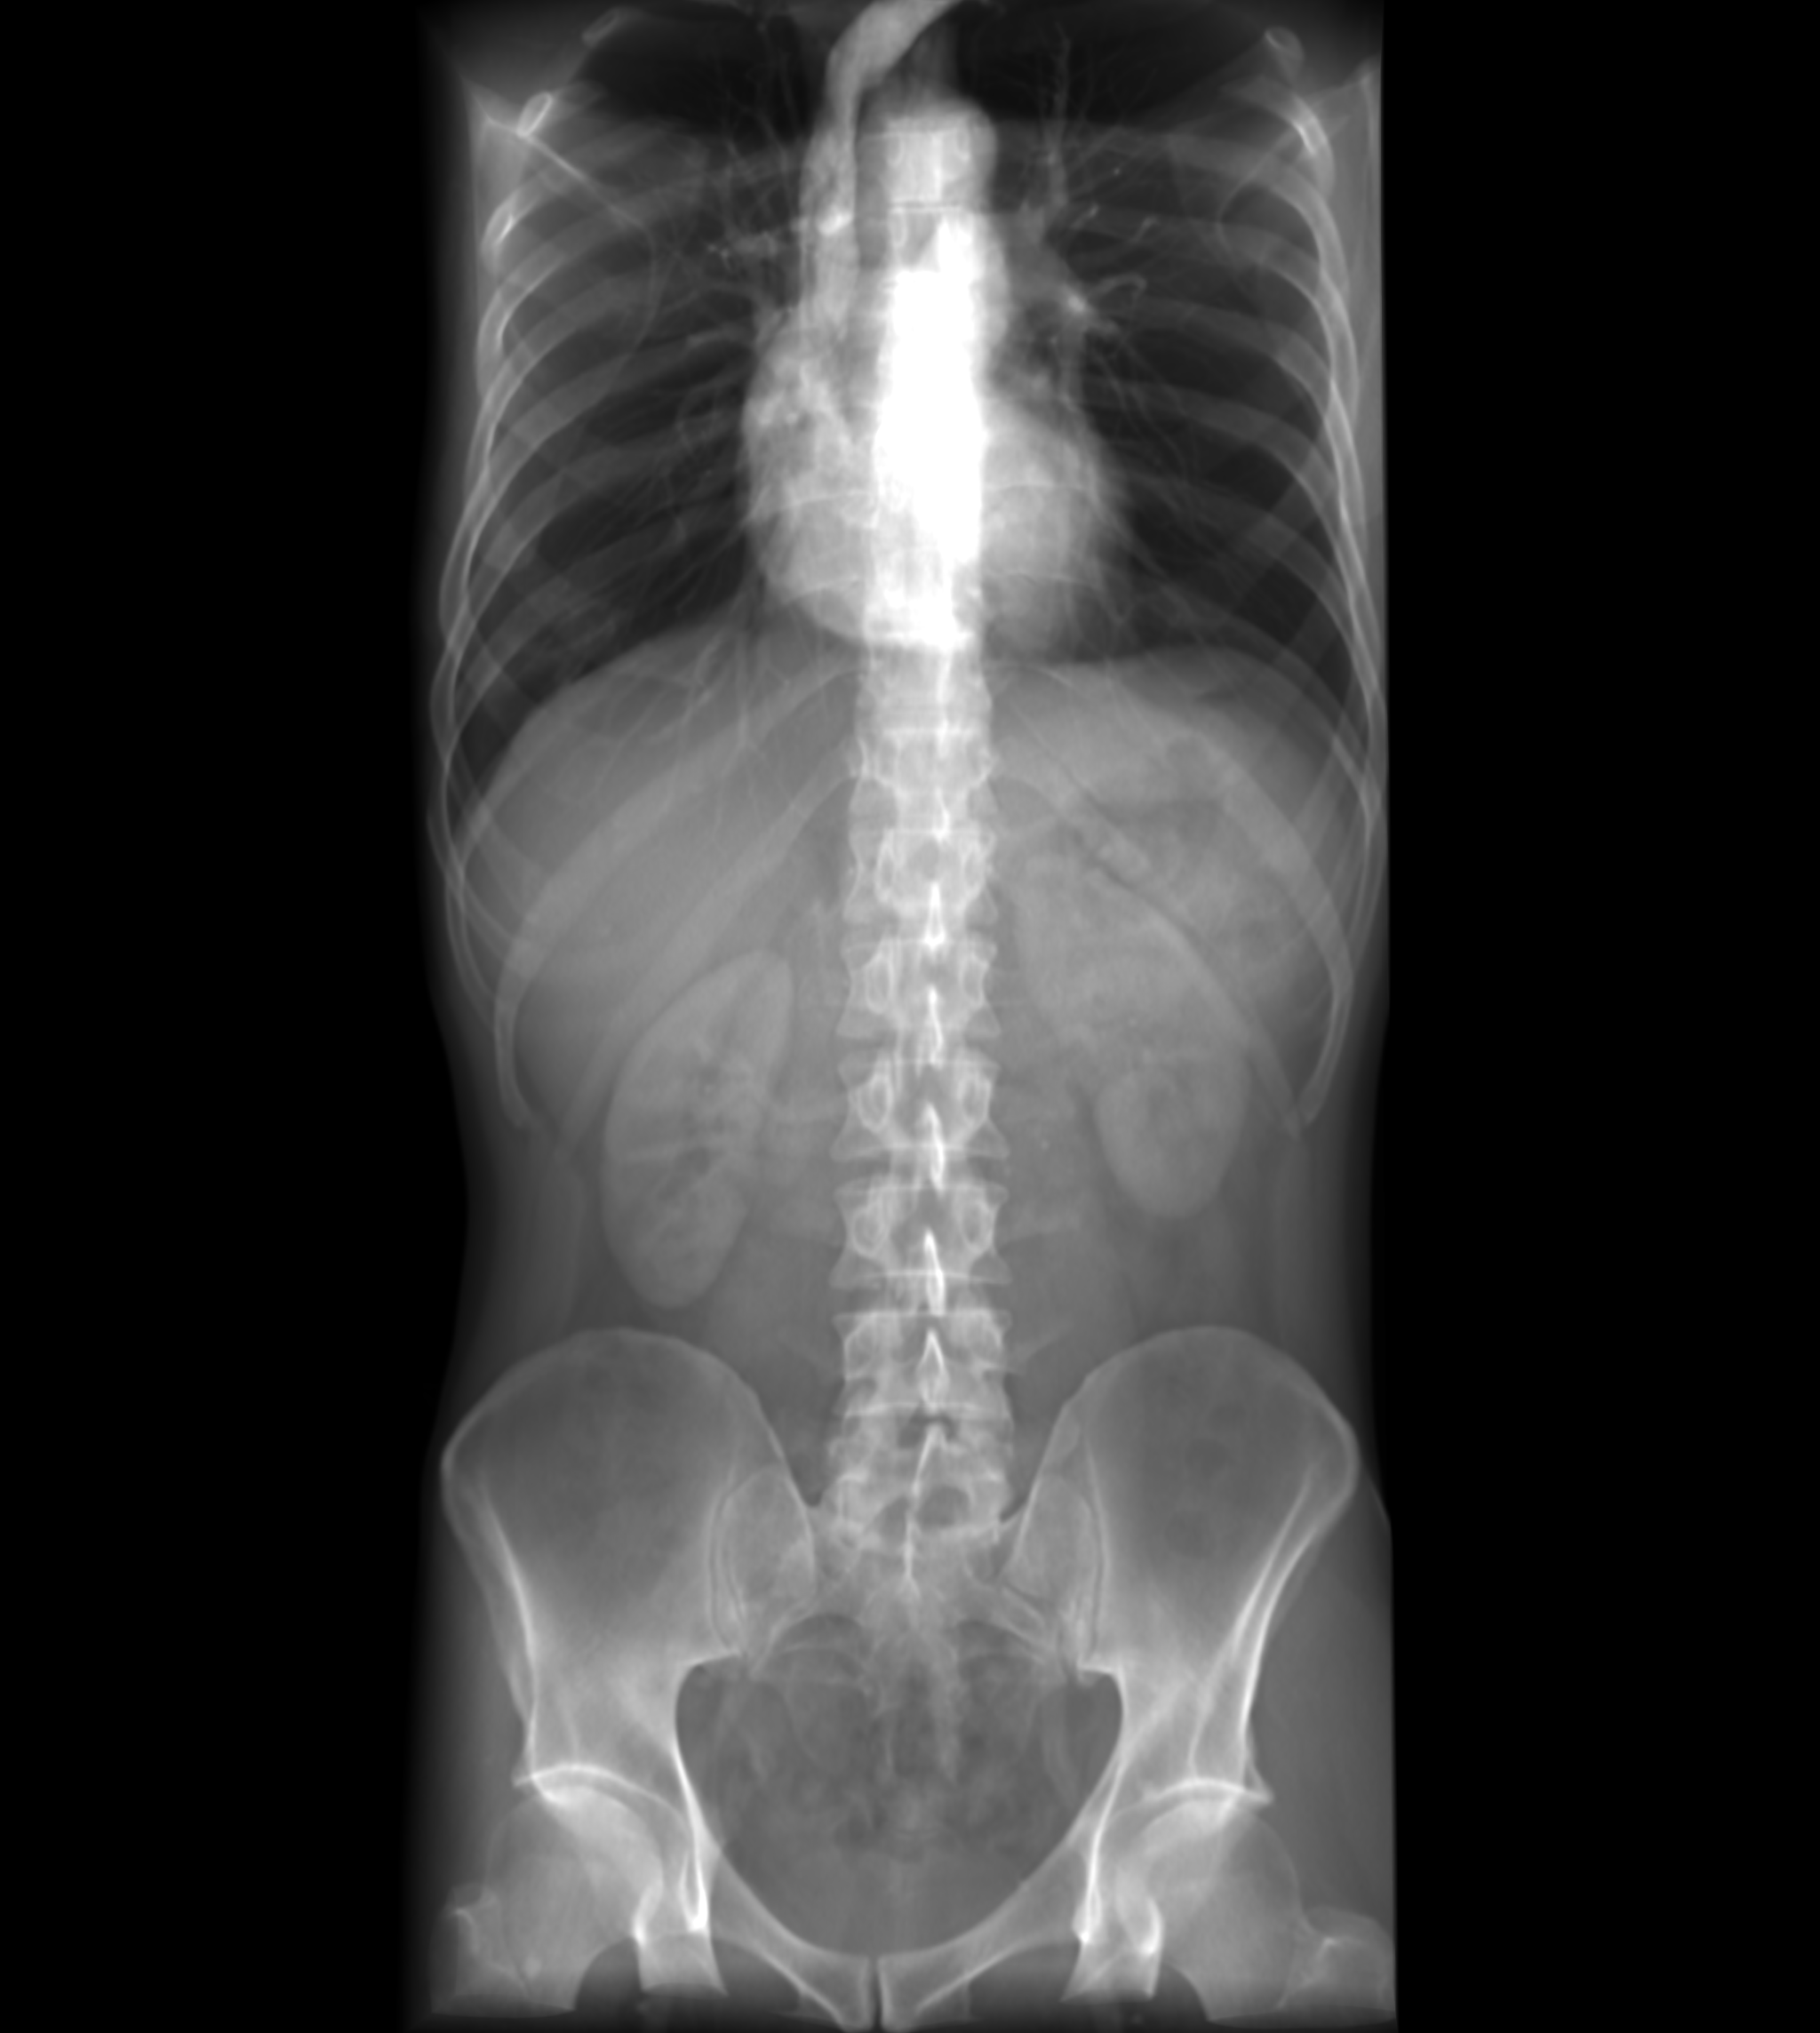
\includegraphics[width=\columnwidth]{TorsoBlendingAdditive}
    \caption{Additive}
    \label{fig:blendadditive}
  \end{subfigure}%
  \begin{subfigure}{.5\columnwidth}
    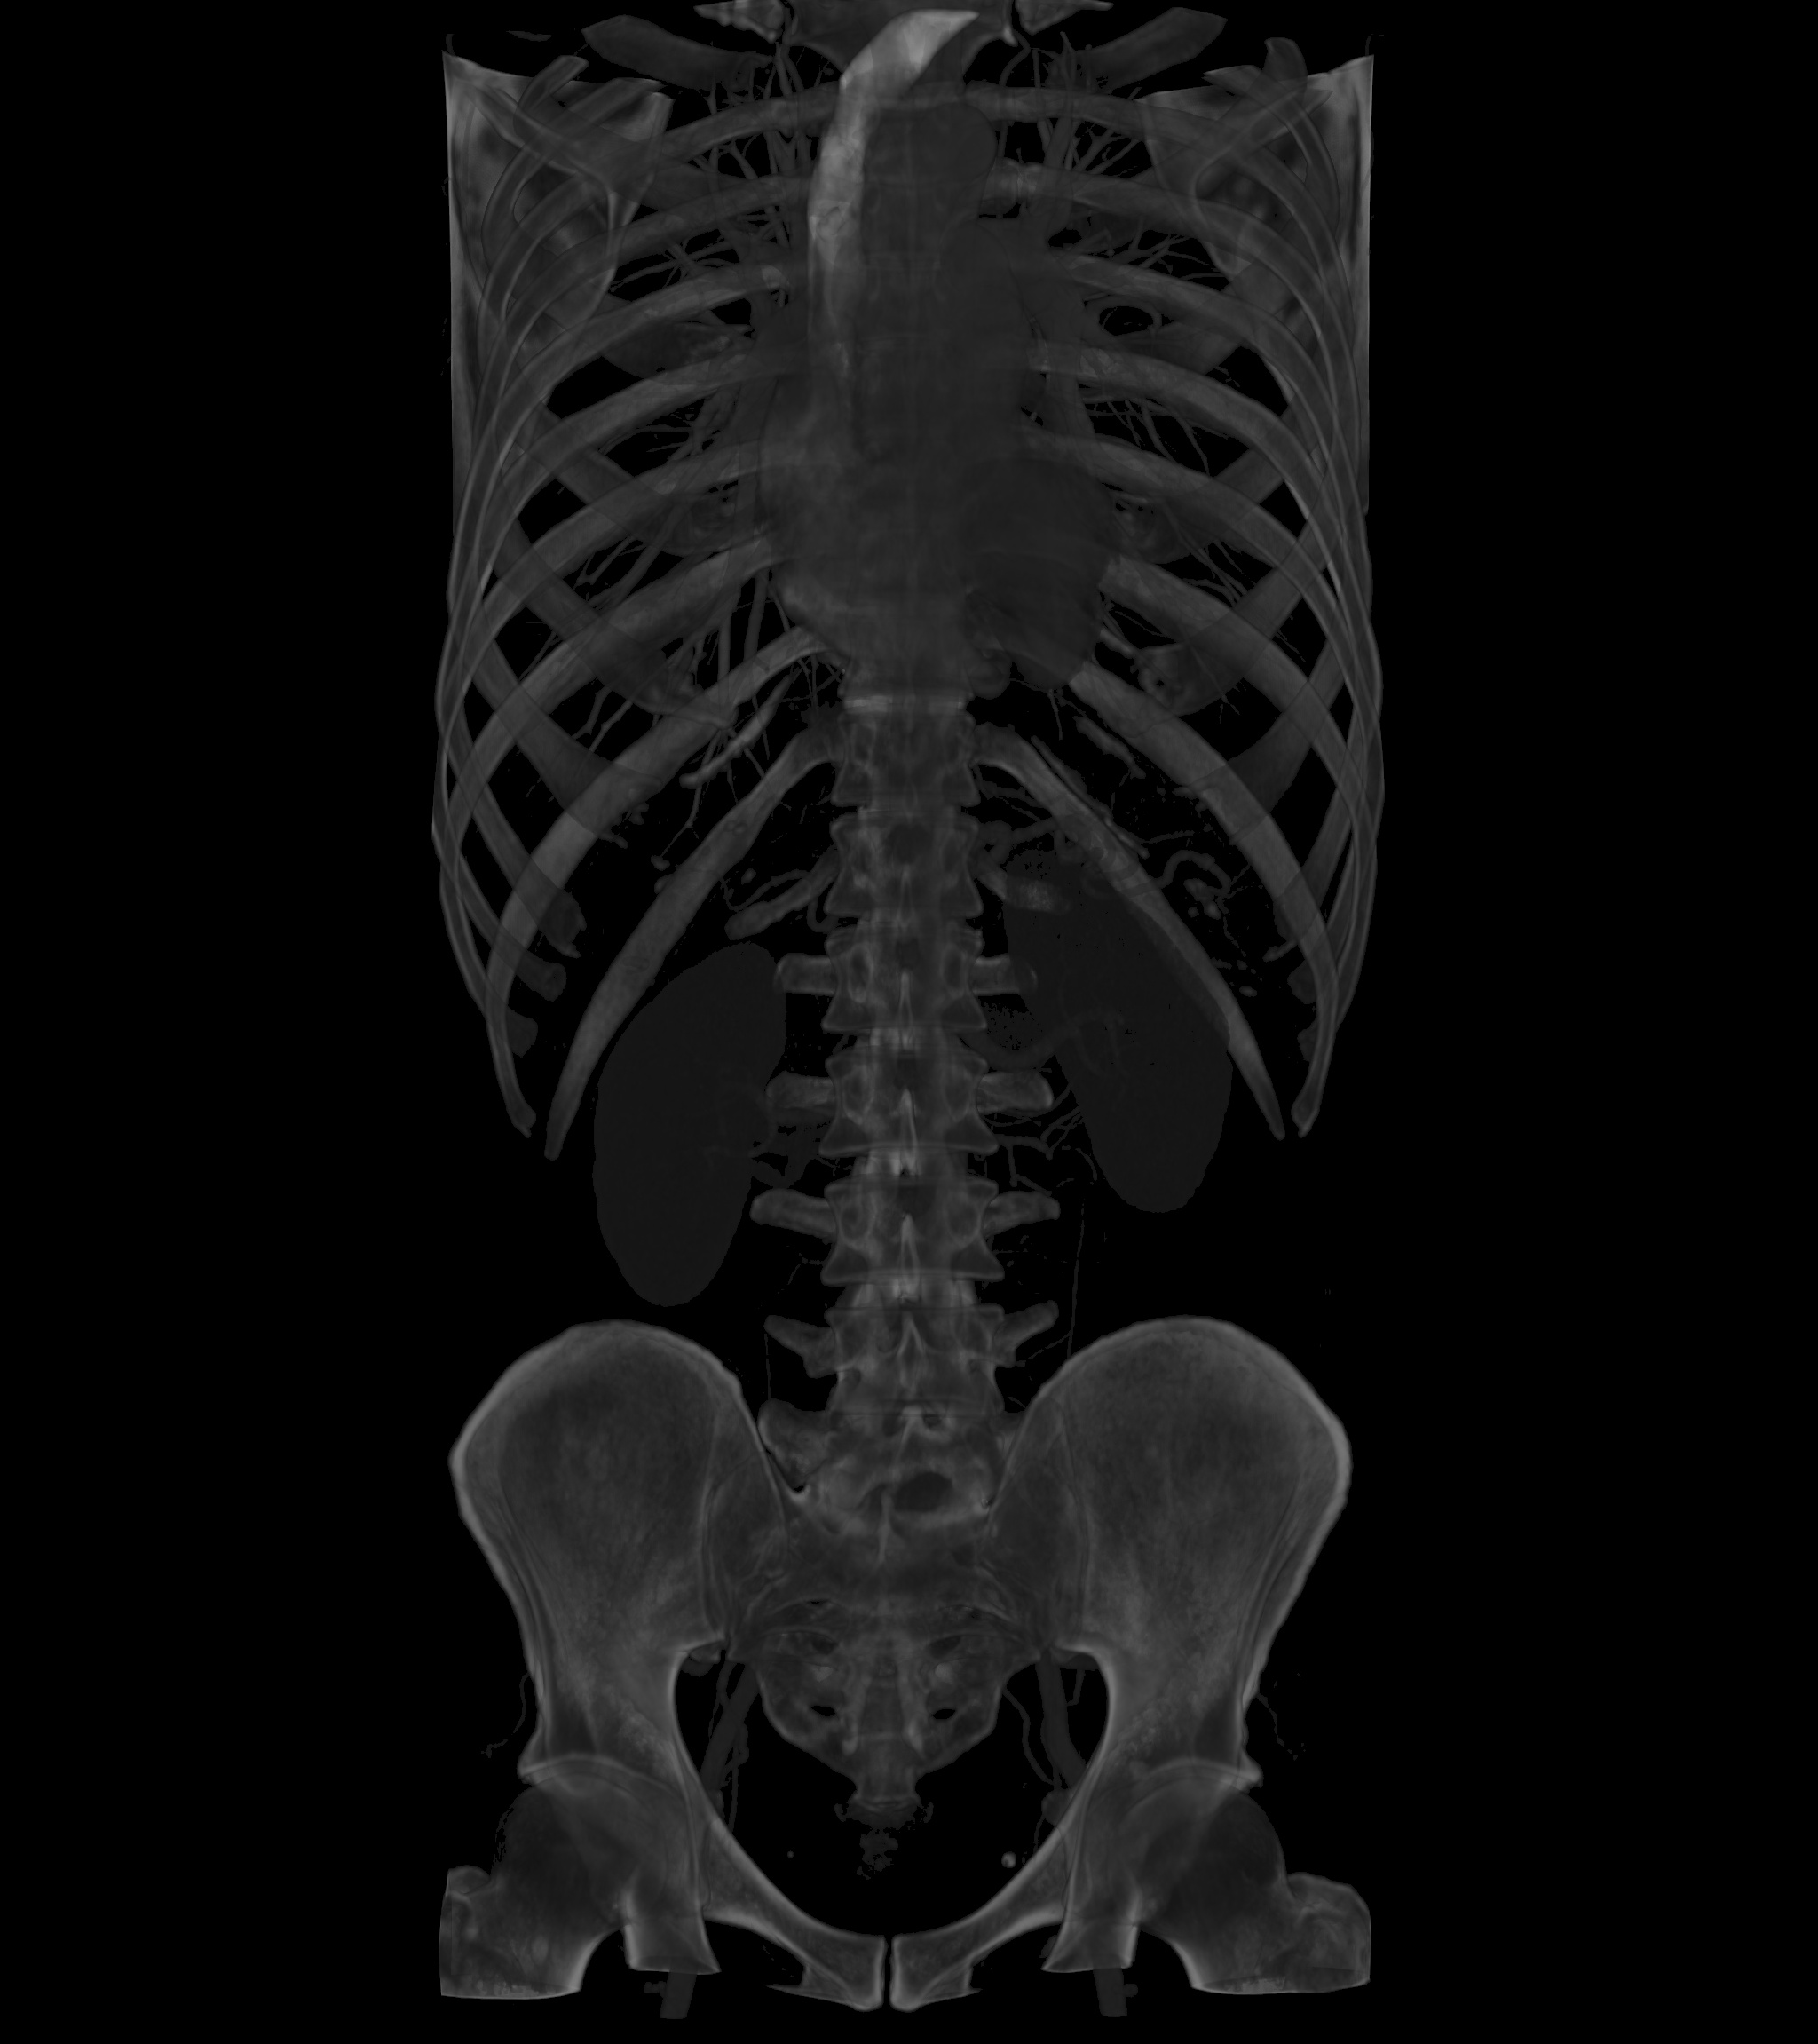
\includegraphics[width=\columnwidth]{TorsoBlendingAverage}
    \caption{Average Intensity}
    \label{fig:blendaverage}
  \end{subfigure}%
  \caption{Blend modes supported by \texttt{vtkGPUVolumeRayCastMapper}}
  \label{fig:blendingmodes}
\end{figure}

\subsection{Masking}
\label{masking}
Both binary and label masks are supported. With binary masks, the value in the
masking volume indicates visibility of the voxel in the data volume. When a
label map is in use, the value in the label map is used to select different
rendering parameters for that sample.  See~\Autoref{fig:rendertotexture}for an
example of label data masks.

\subsection{Opacity Modulated by Gradient Magnitude}
\label{opacity-modulated-by-gradient-magnitude}
While the~\texttt{vtkGPUVolumeRayCastMapper} supports direct accumulation of
color and opacity values along the ray, it also allows for modulating the
opacity accumulation calculation based on relative values of each voxel in the
dataset. Prior efforts~\citep{marchesin_per-pixel_2010} have demonstrated the
usefulness of such a technique for feature enhancement in the rendered image. A
transfer function mapping the magnitude of the gradient to an opacity modulation
value can be used to essentially perform edge detection (de-emphasize homogenous
regions) during rendering. See~\Autoref{fig:gradient} for an example of
rendering with and without the use of a gradient opacity transfer function.

\begin{figure}[htb]
  \centering
   \begin{subfigure}[b]{0.5\columnwidth}
     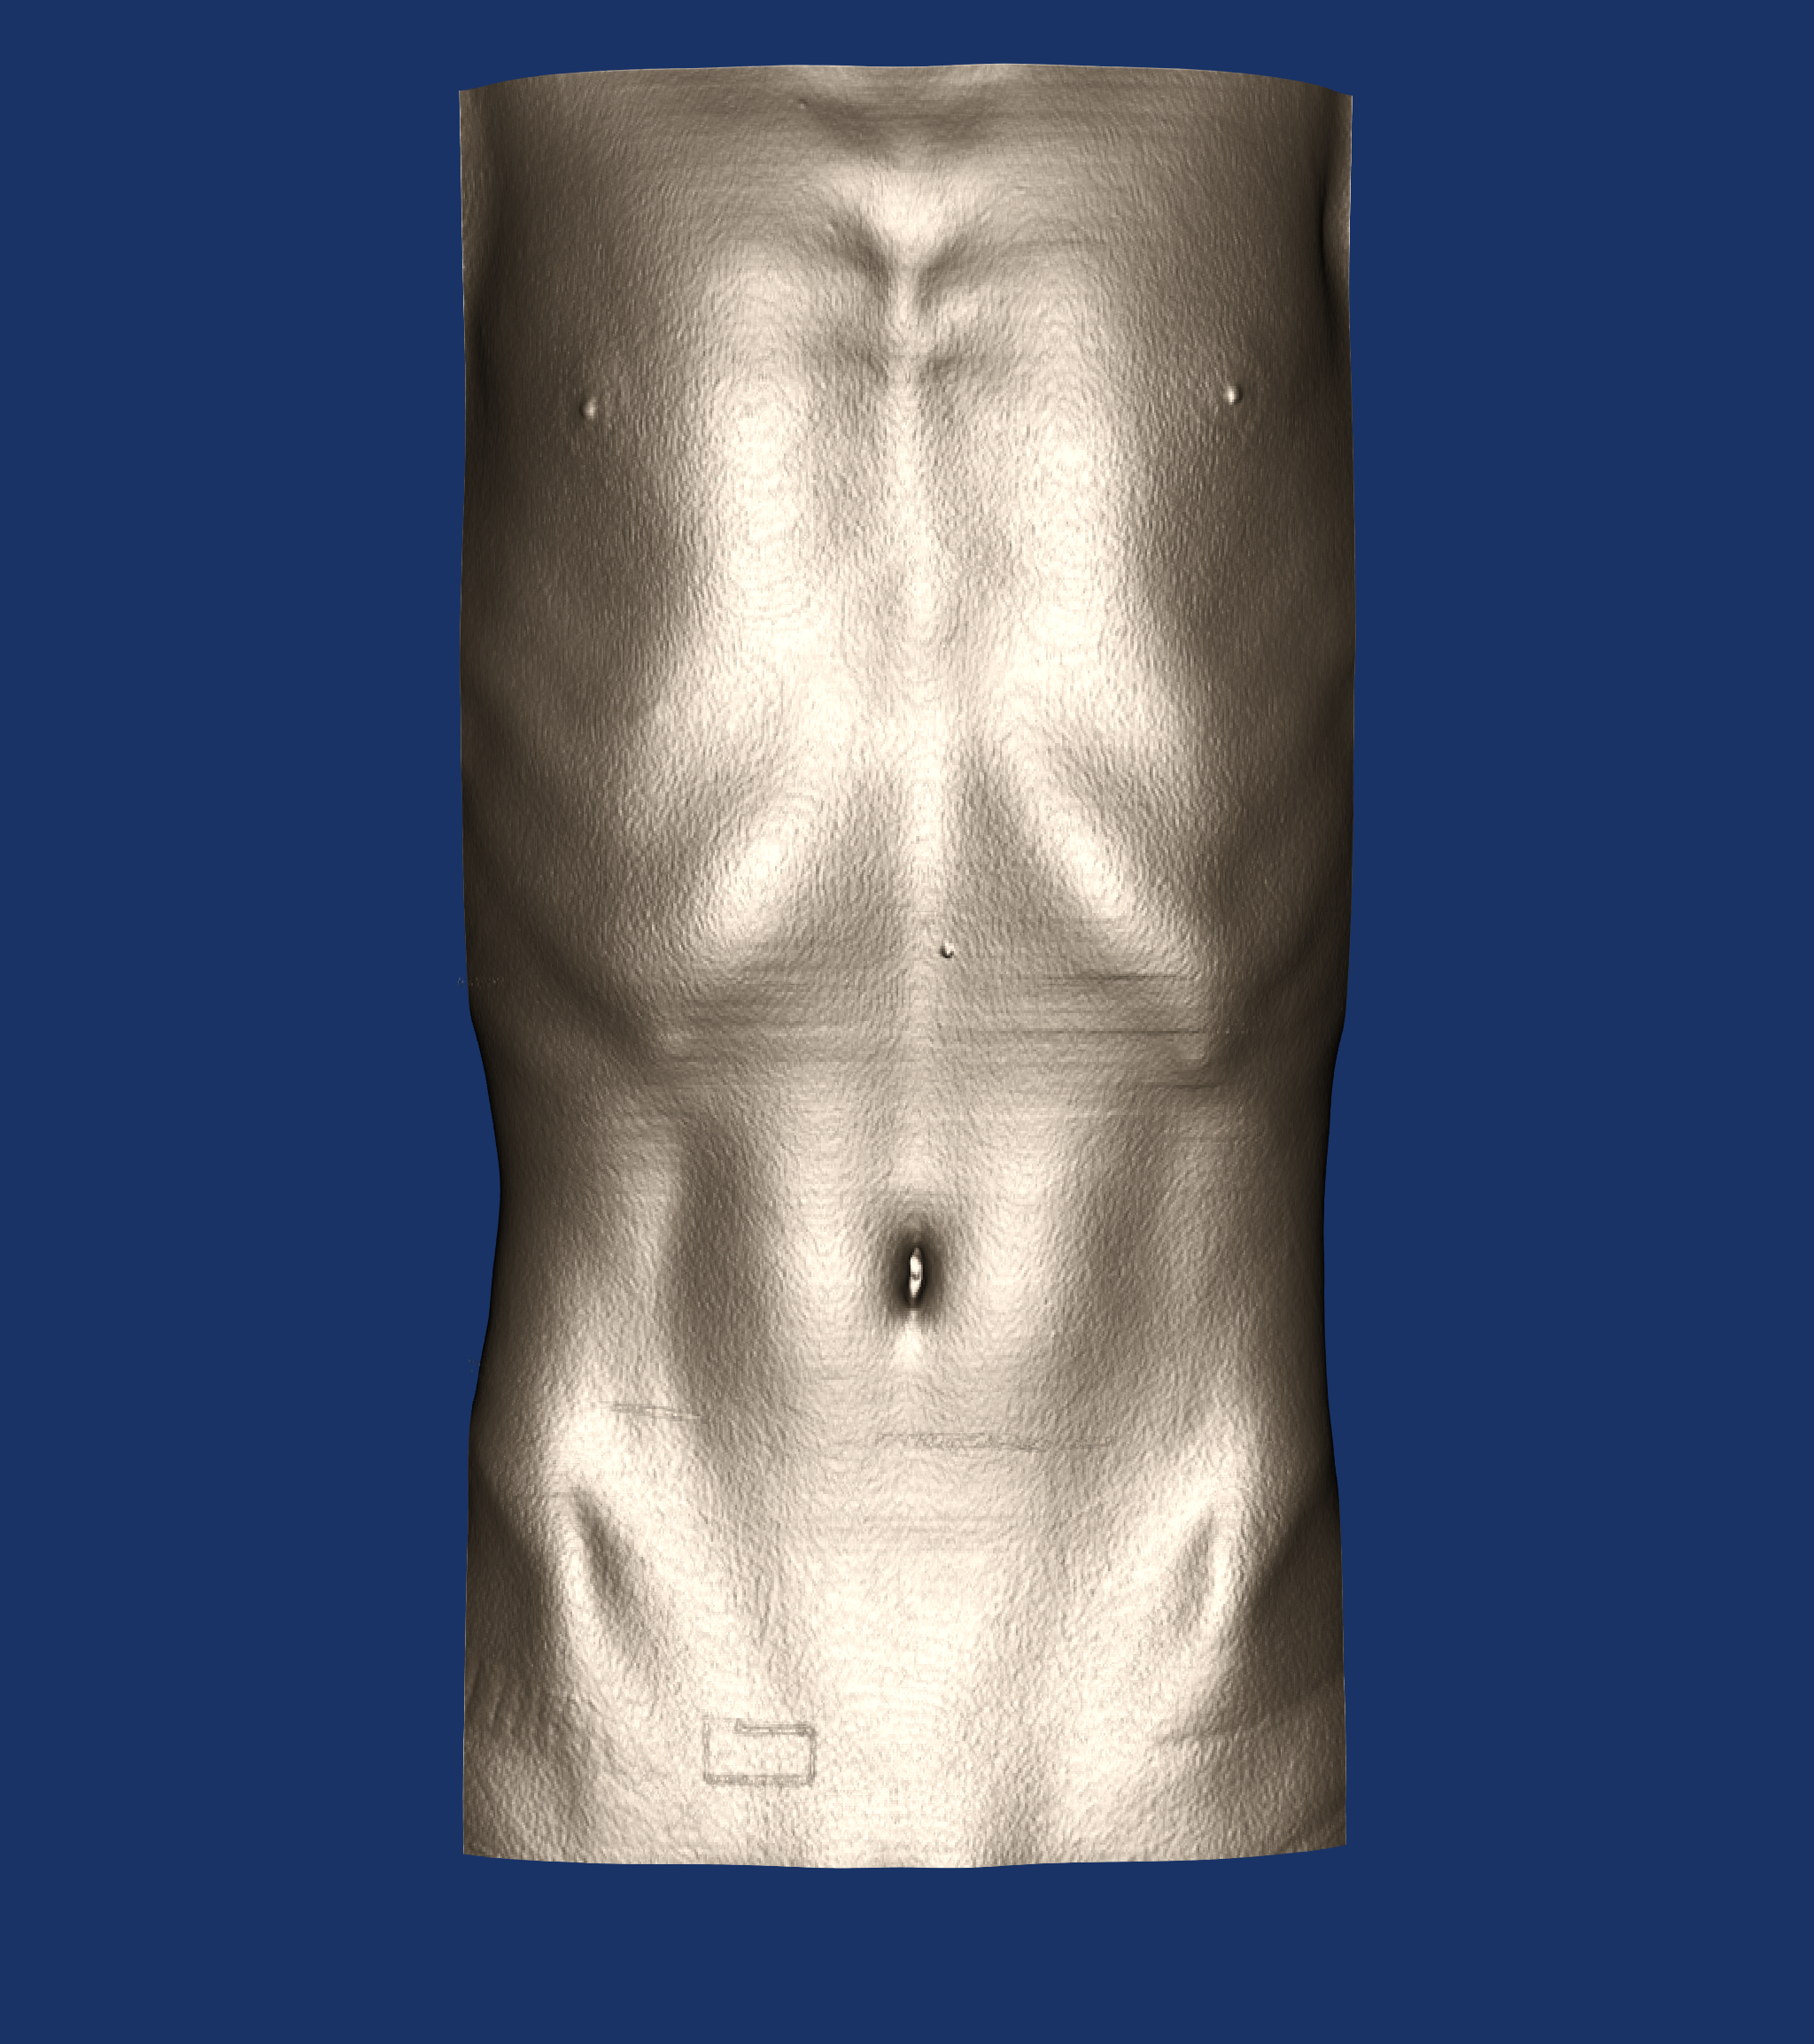
\includegraphics[width=\columnwidth]{TorsoNoGradient}
     \caption{Without gradient opacity}
     \label{fig:Ng1}
   \end{subfigure}%
  \begin{subfigure}[b]{0.5\columnwidth}
    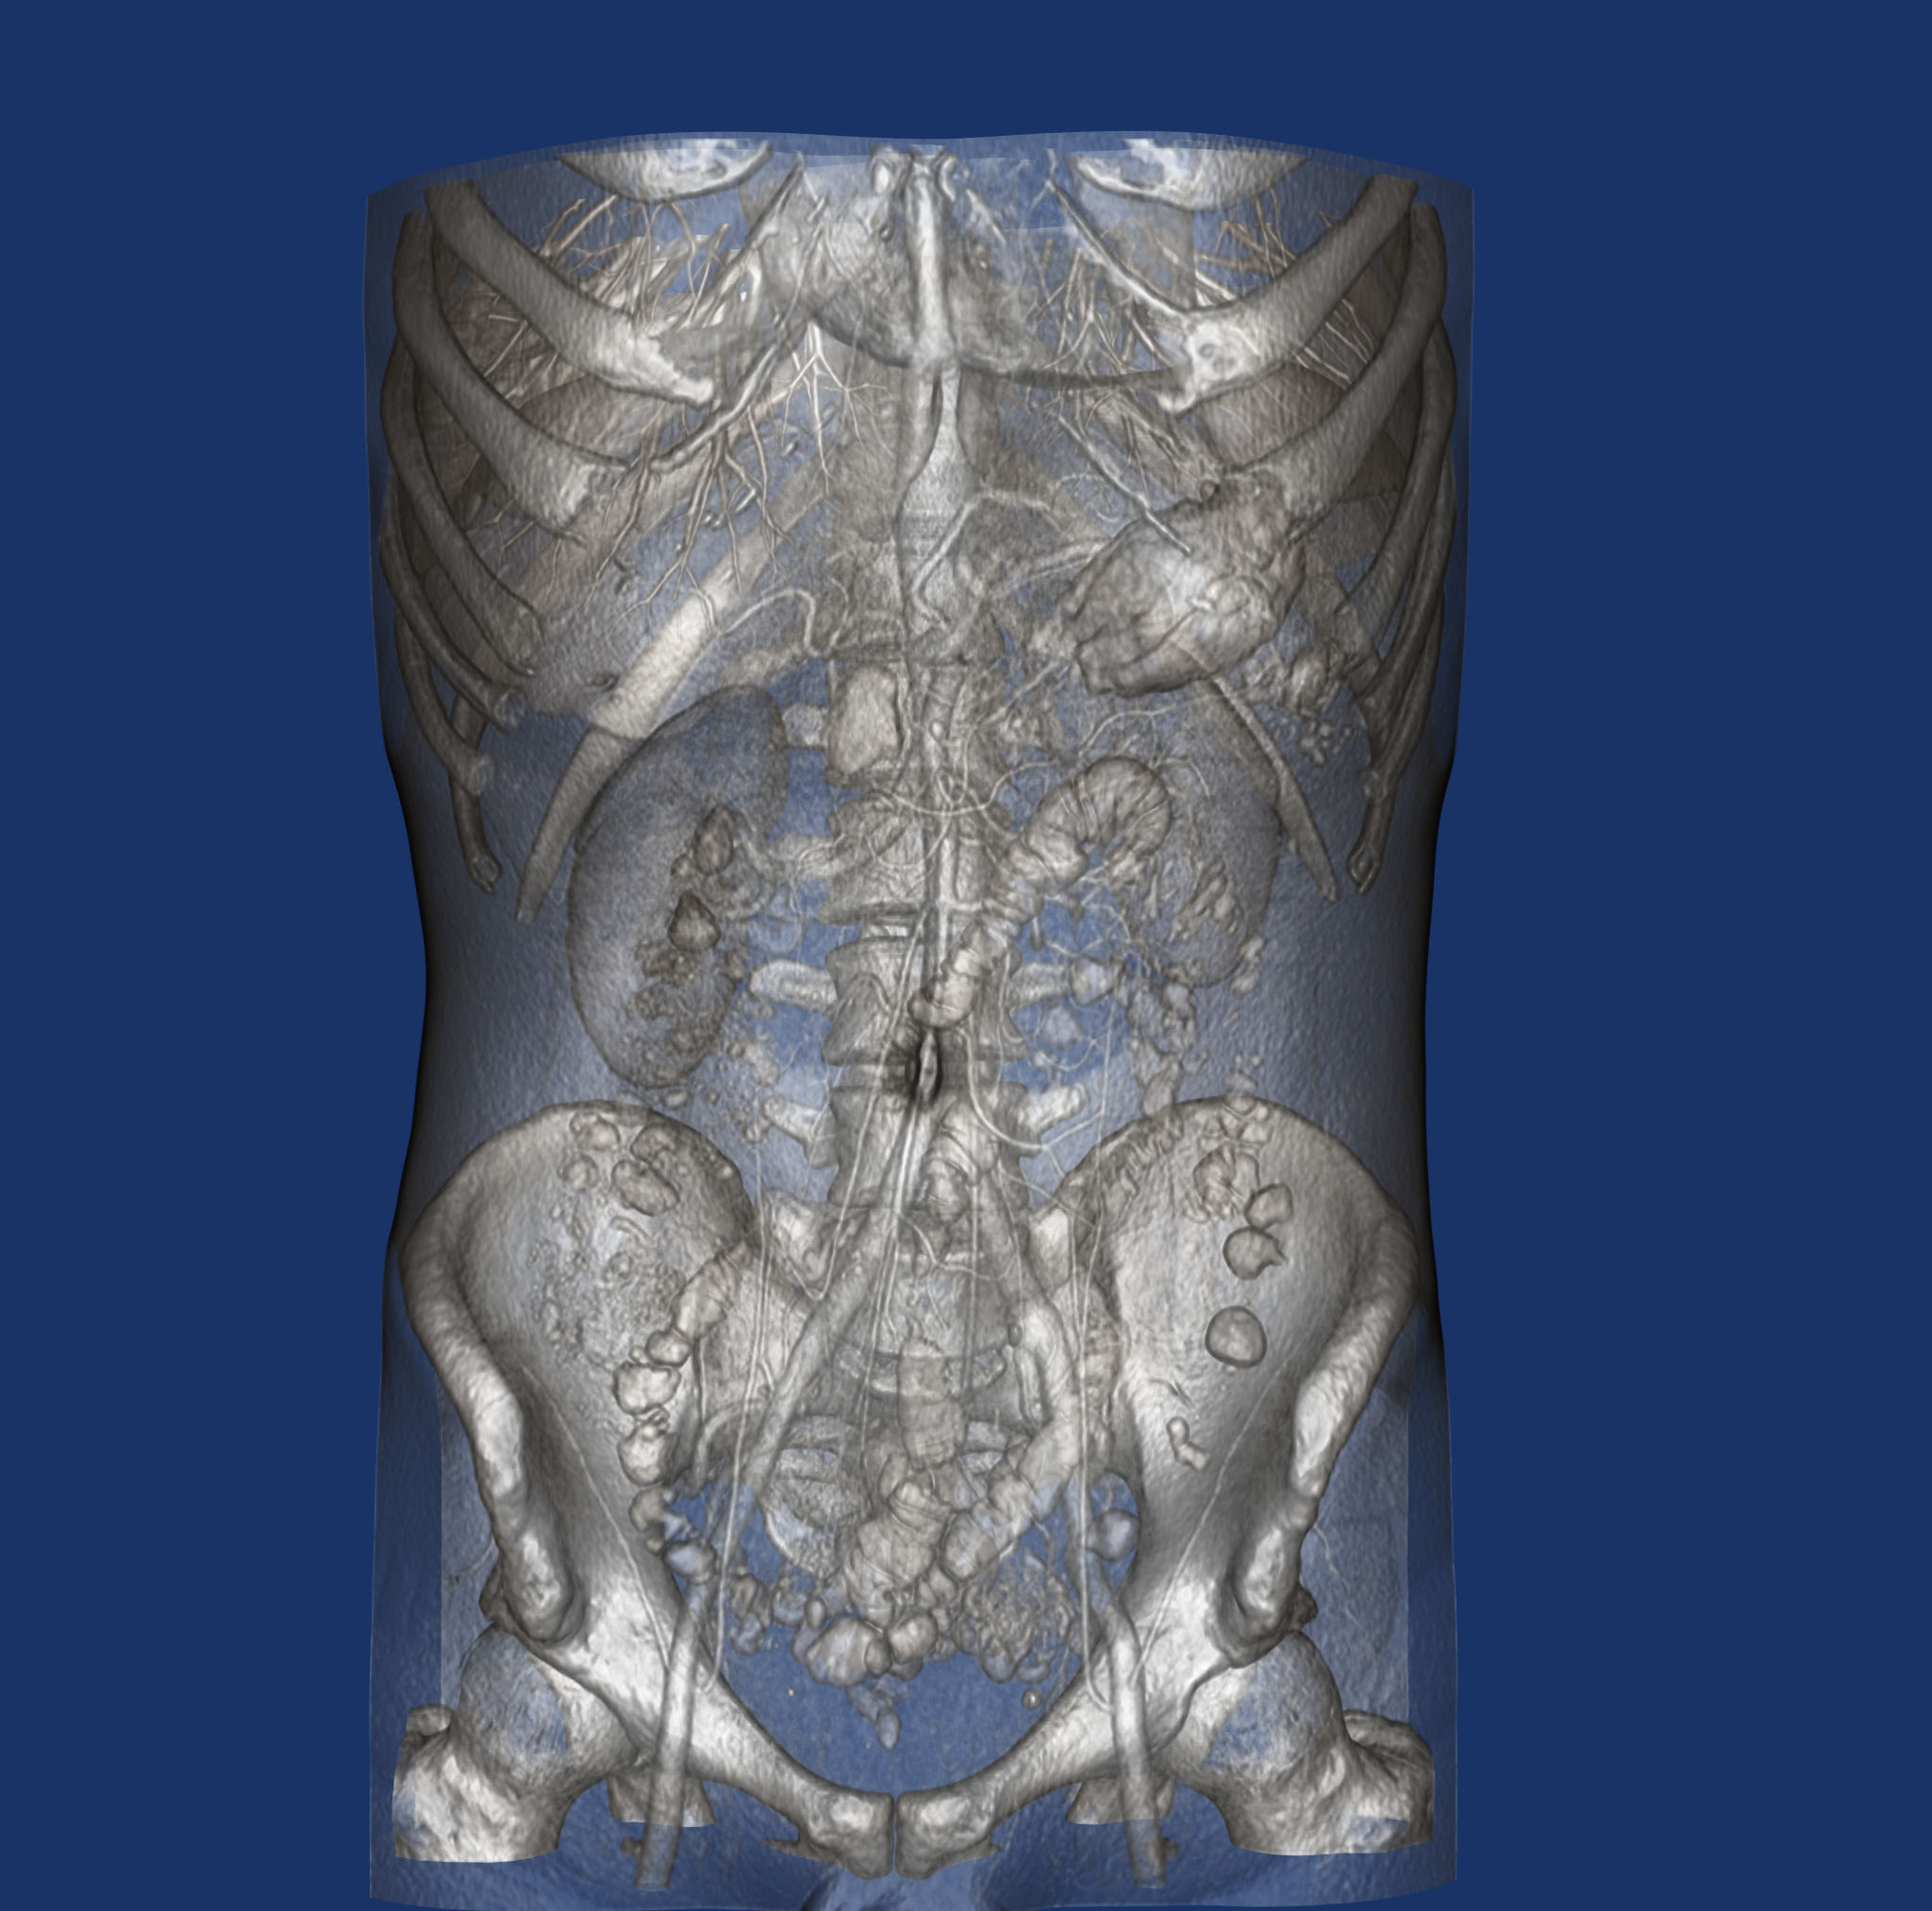
\includegraphics[width=\columnwidth]{TorsoGradient}
    \caption{With gradient opacity}
    \label{fig:Ng2}
  \end{subfigure}
  \caption{Gradient magnitude based opacity modulation}
  \label{fig:gradient}
\end{figure}

\subsection{Optimizations and Edge-Cases} The new
\texttt{vtkOpenGLGPUVolumeRayCastMapper} is more than just a ray cast mapper
implementation. It is designed to work on multiple platforms and developed to
perform volume rendering at interactive frame rates. To achieve interactive
frame rates and to handle edge cases, we have implemented following
optimizations in the new mapper.

\begin{itemize}
  \item \emph{Clipping plane optimization} In VTK, a user can place multiple
    planes at desired angles to clip the volume. This technique is essential for
    many medical use-cases. Since only one side of clip planes needs to be
    traversed, performing any sort of ray cast on the clipped side is wasteful.
    Hence, a simple optimization is to move the starting point of the ray on the
    plane by projecting the ray onto the plane in the view direction.
  \item \emph{Camera Inside the Bounding Box} Rendering with camera views within
    the volume is handled by clipping the proxy geometry with the camera near
    plane (using \texttt{vtkClipConvexPolyData}), thus ensuring that all
    bounding box fragments fall within range.  The Plane-Axis-Aligned-Bounding-Box
    intersection is used to determine whether geometry clipping is necessary.
  \item \emph{Support for Double and Long Long Data Type} The current OpenGL API
    does not support 64-bit data types. In order to be able to render volumes of
    these types, the mapper loads the data array slice by slice casting the data
    values to floating-point. This, despite the obvious precision loss, is
    provided to the user as a convenience feature.
\end{itemize}
